%Dokumentklasse
\documentclass[a4paper, ngerman, 12pt]{scrartcl}

%Seitenränder
\usepackage[top = 2.5 cm, left= 3.5cm, right = 2.5cm, bottom = 3 cm]{geometry}

%Zeilenabstand
%\usepackage[onehalfspacing]{setspace}

% ==== Packages ====

%Dokumentinformationen
\usepackage[
	pdftitle={},
	pdfsubject={},
	pdfauthor={Thomas Zenger},
	pdfkeywords={},	
	%Rahmen von Links verbergen
	hidelinks
]{hyperref}


%Standard Packages
\usepackage[utf8]{inputenc}
\usepackage[T1]{fontenc}
\usepackage{lmodern}
\usepackage{lipsum}


\usepackage{babel}
\usepackage{color, colortbl}
\usepackage{graphicx, subfig}

\usepackage{textcomp}
\usepackage{listings}

\usepackage{amssymb} 
\usepackage{mathtools}

\usepackage{fancyhdr}

\usepackage{svg}
\usepackage{caption}
\usepackage{adjustbox}


\usepackage{hyperref}

\hypersetup{pdftitle={Projektdokumentation Krankentransport}, pdfauthor={Thomas Zenger}, linktoc=all, hidelinks}

%nicht einrücken nach Absatz
\setlength{\parindent}{0pt}

%Trennung
%\hyphenation()

%Redefine
\renewcommand{\headrulewidth}{0.4pt}
\renewcommand{\footrulewidth}{0.4pt}

% ==== Kopf- und Fußzeile ====
\pagestyle{fancy}
\fancyhf{}
\lhead{}
\chead{}
\rhead{\leftmark}
%%
\lfoot{Projektdokumentation Krankentransport}
\cfoot{}
\rfoot{\thepage}
%%



\begin{document}

%Titelseite
\begin{titlepage}
\begin{center}
\begin{flushleft}

\includegraphics[height=30mm]{def/OTHR_FakIM_Logo}
\end{flushleft}
\vspace*{3cm}
{\Huge\textbf{Projektdokumentation}}\\
\vspace{1cm}
{\huge Krankentransport}\\
\end{center}
\vspace{\fill}
%Author
\begin{normalsize}
\begin{tabular}{p{4cm}p{4cm}p{4cm}}
Eingereicht von:	&Brunner Sebastian		&3130364\\
				&Klamer Florian		&\\
				&Richter Felix			&\\
				&Winter Tobias			&\\
				&Zenger Thomas		&3073975\\
\end{tabular}\\[0.5em]
\begin{tabular}{p{4cm}p{6cm}}
Studiengang:		&Informatik			\\[0.3em]
Kurs:				&Human Comuter Interaction	\\
				&Wintersemester 2019/2020	\\[0.3em]
Betreuer:			&Prof. Dr. Markus Heckner	\\
\end{tabular}\\[3em]
Regensburg, den \today
\end{normalsize}
\vspace{1cm}
\end{titlepage}


\pagestyle{fancy}
%Inhaltsverzeichnis
\tableofcontents
\newpage

%Verzeichnis aller Bilder
\listoffigures
\newpage

%Verzeichnis aller Tabellen
%\listoftables
%Verzeichnis aller Code Listings
%\lstlistoflistings

\section{Einleitung}
Nach einem Krankenhausaufenthalt will jeder wieder nach Hause. Wer jedoch nicht selbst fahren oder gehen kann, muss die Möglichkeit eines Krankentransportes in Anspruch nehmen. Auch wenn ein Patient in ein anderes Krankenhaus verlegt werden muss oder eine Einrichtung zur Rehabilitation besucht, ist ein Krankentransport zu rufen. Obwohl das Bestellen des Transportes sehr zeitaufwendig ist, wird es meist von Mitarbeitern des Krankenhauses erledigt. Dass dies im Zeitalter der digitalen Revolution noch manuell passiert ist, für Informatiker nur schwer verständlich.\\

Immer stärkere, billigere und kleinere Computer erlauben die Digitalisierung alltäglicher Prozesse und ermöglichen die Erschaffung des Internet of Things. Smart Home und Industrie 4.0 zeigen das Potenzial von ubiquitärem Computing, werden jedoch von Vielen kritisch gesehen. Was eigentlich als Unterstützung von Menschen bei alltäglichen Dingen gedacht ist, bedeutet für viele zusätzlichen Aufwand. Bei genauerer Betrachtung stellt sich heraus, dass viele Systeme von den Entwicklern theoretisch gut konzipiert sind, jedoch in der Praxis keine Akzeptanz finden. Diese Diskrepanz zwischen Theorie und Praxis liegt häufig in der schlechten User Experience. Software wird auch heute noch häufig entwickelt, ohne auf die Bedürfnisse des Endnutzers einzugehen. 
\section{Projektbeschreibung}
Dieses Projekt soll zu der erfolgreichen digitalen Transformation des Krankenhauses beitragen, indem mit Hilfe von Usercentered Design eine Basis für ein benutzerfreundliches System erarbeitet wird, welches den Prozess des Krankentransportes verbessert bzw. die Beteiligten unterstützt. Dafür wird der gesamte End-to-end-Prozess des Krankentransportes betrachtet. Dieser beginnt mit der Entscheidung, dass ein Patient verlegt oder entlassen wird und endet mit der Ankunft des Patienten am Ziel. Dabei soll nicht nur auf die Bedürfnisse medizinischer Einrichtungen und Patienten eingegangen werden, sondern auch auf die der Transportunternehmer.\\

Über eine Kooperation der OTH Regensburg mit der Abteilung Healthcare der BioPark Regensburg GmbH unter der Aufsicht von Prof. Dr. Markus Heckner und Dr. Ilja Hagen soll ein passendes Usability-Konzept erstellt und am konkreten Nutzer getestet werden. Healthcare Regenburg untersucht z.Z. die Möglichkeit, wie Transportunternehmen über eine Zentrale mit Krankenhäusern vernetzt werden können, um Krankentransporte effizient zu planen. Der Hauptfokus dieses Projekts liegt hierbei in der User Experience der Mitarbeiter im Krankenhaus.
\newpage
\section{Methoden}
\begin{figure}[h]
	\centering
	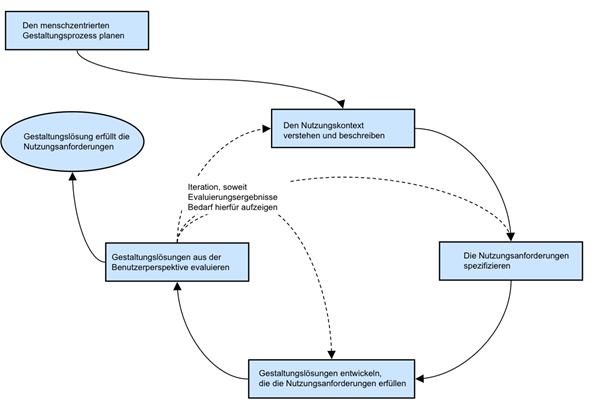
\includegraphics[width=0.8\textwidth]{../Bilder/9241-210.png}
	\caption{Bild 1 aus DIN EN ISO 9241-210: Wechselseitige Abhängigkeit menschzentrierter Gestaltung Aktivitäten}
	\label{img:9241-210}
\end{figure}
In diesem Projekt werden verschiedenste Methoden angewandt, um die Qualität des Designs zu sichern.\\

Es werden nicht nur die Vor- und Nachteile des existierenden Prozesses analysiert, sondern auch von existierenden Softwarelösungen. Diese Vor- und Nachteile fließen in die Anforderungsanalyse mit ein.\\

Zur Konzipierung wird nach dem iterativen „Prozess zur Gestaltung gebrauchstauglicher Systeme“ (ISO 9241-210) vorgegangen. Dieser besteht neben der Planung aus einem Zyklus, welcher sich aus der Analyse des Nutzungskontexts, Spezifikation der Anforderungen, Implementierung und Evaluation zusammensetzt. In den einzelnen Schritten wird eine Auswahl verschiedener Methoden aus dem Usercentered Design verwendet. Wegen des Fachkräftemangels im Gesundheitswesen kann nur wenig Pflegepersonal für die Durchführung der Anforderungsanalyse abgestellt werden. Somit entfallen Methoden, für die viele Testpersonen benötigt werden. Der gesamte Projektablauf wird mit einem Kanban-Board der App „Trello“ und einem Gannt-Diagramm der App „teamgannt“ geplant und überprüft.\\

\begin{minipage}{\textwidth}
	\centering
		\includesvg[width=\textwidth]{../Bilder/ProjektplanTeil1.svg}
		\captionof{figure}{Projektplan Krankentransport - Teil 1}
		\label{img:projektplan1}
\end{minipage}\\[0.5em]

\begin{minipage}{\textwidth}
	\centering
	\includesvg[width=\textwidth]{../Bilder/ProjektplanTeil2.svg}
	\captionof{figure}{Projektplan Krankentransport - Teil 2}
	\label{img:projektplan2}
\end{minipage}\\[0.5em]

\begin{minipage}{\textwidth}
	\centering
	\includesvg[width=\textwidth]{../Bilder/Arbeitsaufteilung.svg}
	\captionof{figure}{Arbeitsaufteilung}
	\label{img:arbeitsaufteilung}
\end{minipage}\\[0.5em]

\begin{minipage}{\textwidth}
	\centering
	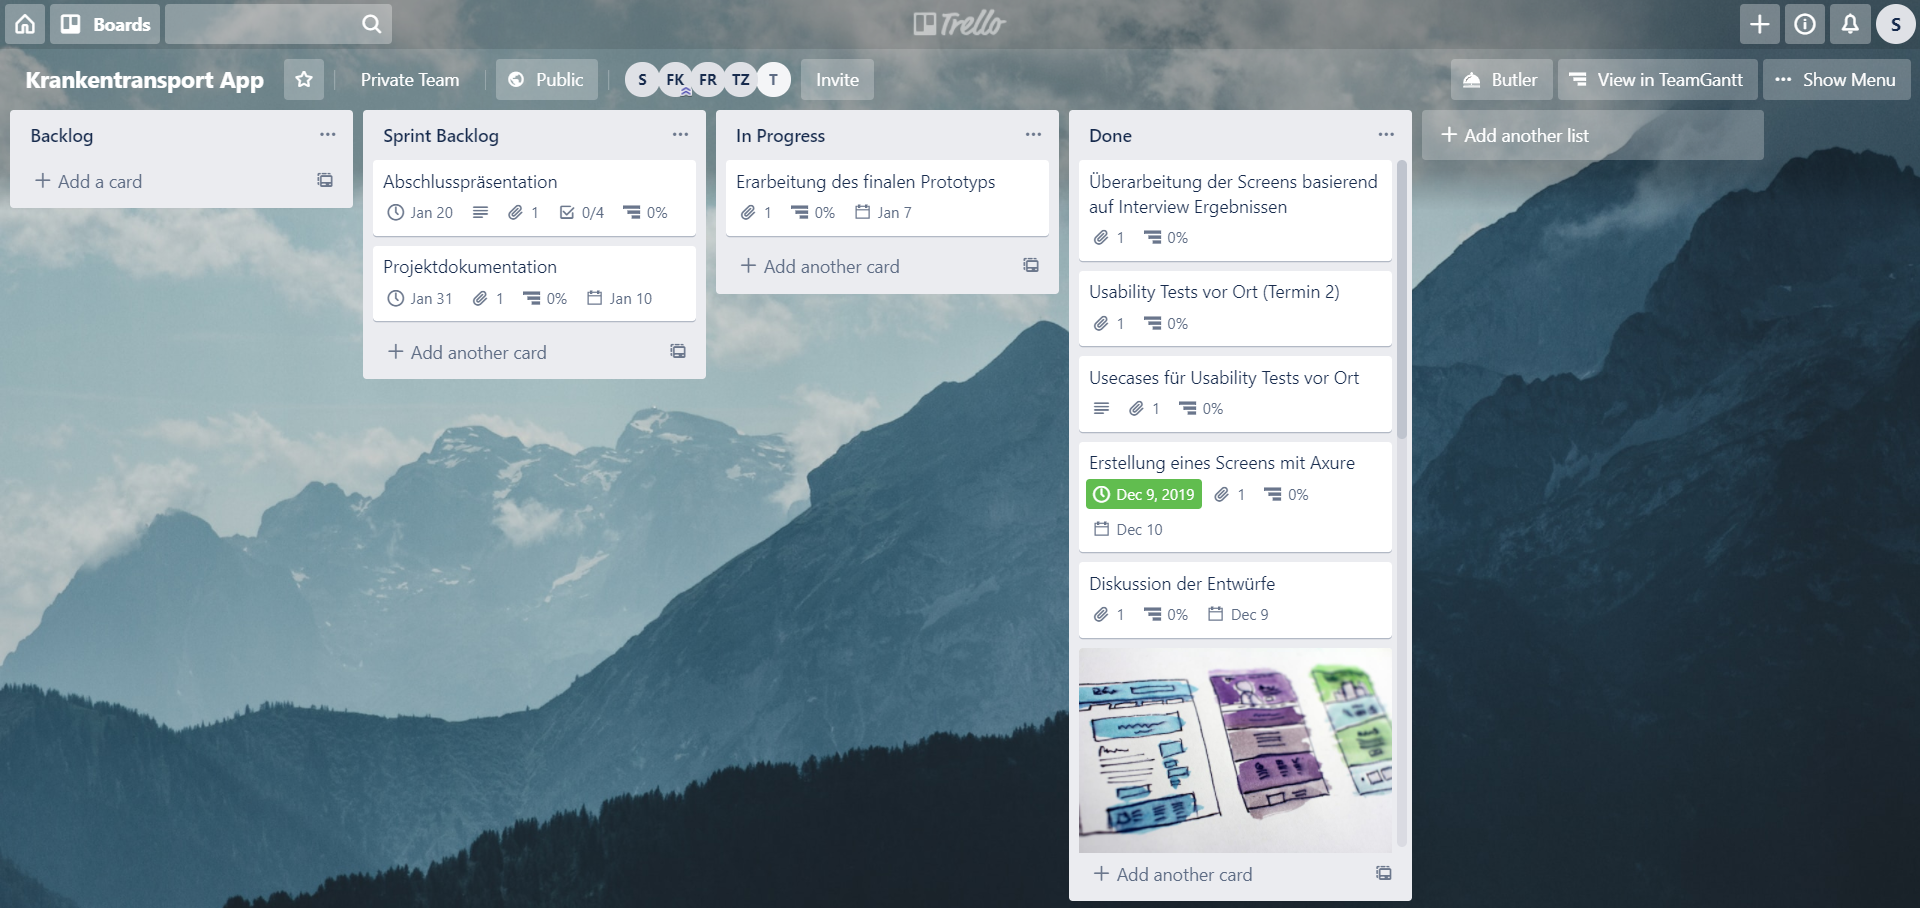
\includegraphics[width=\textwidth]{../Bilder/trelloboard.png}
	\captionof{figure}{Trello Board}
	\label{img:trello}
\end{minipage}\\
\newpage
Es werden folgende Methoden aus dem Usercentered Degsign angewandt:
\begin{itemize}
\item \textit{Interviews} zeigen die Mängel im bestehenden Prozess, welche Krankenhausmitarbeitern am ehesten auffallen. Viele Probleme werden jedoch nicht bewusst erkannt.
\item Durch  \textit{Contextual Inquiries} werden nicht direkt wahrgenommene Probleme herausgefunden. Schwestern werden bei ihrer Arbeit begleitet um so die Praxis auch aus externer Sicht zu beurteilen.
\item User Requirements werden anhand von  \textit{Personas} und  \textit{Requirement Lists} festgelegt.
\item Durch  \textit{Sketching} werden verschiedene Varianten eines  \textit{Papierprototypen} erstellt und von den Entwicklern bewertet. Die dadurch entstandenen Ideen werden in einem einzigen Papierprototypen vereinigt.
\item Dieser wird digitalisiert und in Form eines  \textit{High-Fidelity-Prototypen} direkt mit dem User getestet.
\end{itemize}
Nicht verwendet werden z.B.  \textit{Fokusgruppen} oder  \textit{Surveys}, da dafür vom Krankenhaus nicht genügend  \textit{Human Resources} gestellt werden können.\\

\section{Evaluation des Nutzungskontexts}
\subsection{Personas}
\subsubsection{Krankenschwester (Bezirksklinikum)	}
Die Krankenschwestern auf Station sind für die Bestellung der Krankentransporte zuständig. Allmorgentlich findet eine Besprechung mit den behandelnden Ärzten statt. Dabei wird gemeinsam über die Entlassung der Patienten entschieden. Wird ein Patient entlassen, so drucken die Schwestern einen Adressaufkleber, der auf dem Formblatt über die Fahrdienstleistung aufgeklebt wird. Die restlichen Punkte des Formblattes werden handschriftlich ausgefüllt.\\
Nachdem das Formblatt vervollständigt ist, wird es vom Arzt unterschrieben und telefonisch die Organisation des Transportes beim hauseigenen Fahrdienst angefordert.
\subsubsection{Arzt}
Der Arzt ist weitestgehend vom eigentlichen Prozess entkoppelt. Er gibt lediglich seine Zustimmung zur Entlassung, welche dann von den Schwestern durch einen Stempel auf dem Fahrdienstleistungsformblatt bestätigt wird.
\subsubsection{Fahrdienst (Bezirksklinikum)}
Der Fahrdienst erhält die Transportanfragen der einzelnen Stationen und kümmert sich um die Disposition der Fahrten im Bezirksklinikum. Die Anfragen werden telefonisch übermittelt und auf Papier festgehalten.
\subsection{Interview \& Feldbeobachtung}
\colorbox{yellow}{tbi}\\
\section{Anforderungsmanagement}
\subsection{Anforderungsanalyse}
Folgende Tabellen listen die Anforderungen des Projekts auf. Die Anforderungen wurden in funktionale und nicht funktionale Anforderungen unterteilt. Eine Gewichtung verdeutlicht die Priorität der jeweiligen Anforderung. Die Anforderungen wurden aus der Aufgabenstellung und den ersten Interviews zum allgemeinen Ablauf im Krankenhaus St. Josef und dem Bezirksklinikum erarbeitet (Quelle: Entwickler). Anforderungen, die aktiv vom Anwender eingebracht wurden sind mit \texttt{Quelle:User} gekennzeichnet. Abschließend wurde jede Anforderung auf ihre Verifizierbarkeit hin bewertet\\[0.5em]
 \begin{adjustbox}{max width=\textwidth}
\begin{tabular}{|c|l|c|c|c|}
\hline
\rowcolor{lightgray}\textbf{ID}	&\textbf{funktionale Anforderungen}	&\textbf{Quelle}&\textbf{Gewichtung}	&\textbf{verifizierbar}\\
\rowcolor{lightgray}	&						&		&\scriptsize{1 bis 3 absteigend}			&\\
\hline
AF01&Transporte anzeigen						&Entwickler		&1		&Ja\\
\hline
AF01.1&Gruppierung der Transporte						&Entwickler		&3		&Ja\\
\hline
AF02&Informationen zu Transport anzeigen
						&Entwickler		&2		&Ja\\
\hline
AF03&Transporte suchen
						&Entwickler		&2		&Ja\\
\hline
AF04&Rückmeldung zu Status
						&User		&1		&Ja\\
\hline
AF05&Neuer Transport erstellen
						&Entwickler		&1		&Ja\\
\hline
AF06&Patientendaten eingeben
						&Entwickler		&1		&Ja\\
\hline
AF07&Patientendaten importieren
						&User		&2		&Ja\\
\hline
AF08&Bestehende Daten verändern
						&Entwickler		&3		&Ja\\
\hline
AF09&Patientendaten in EPA aktualisieren
						&User		&2		&Ja\\
\hline
AF10&Transportdaten angeben
						&Entwickler		&1		&Ja\\
\hline
AF10.1&Transportart angeben
						&Entwickler		&2		&Ja\\
\hline
AF10.2&Abweichendes Transportziel angeben
						&User		&2		&Ja\\
\hline
AF10.3&Dringlichkeit angeben
						&User		&2		&Ja\\
\hline
AF11&Arztstempel einfügen
						&User		&1		&Ja\\
\hline
AF12&Überprüfung Eingabe
						&Entwickler		&2		&Ja\\
\hline
AF13&Patienten suchen
						&Entwickler		&3		&Ja\\
\hline
AF14&Transportanfrage übermitteln
						&Entwickler		&1		&Ja\\
\hline
AF15&Patient entlassen
						&Entwickler		&3		&Ja\\
\hline
\end{tabular}
\end{adjustbox}\\[1em]
 \begin{adjustbox}{max width=\textwidth}
\begin{tabular}{|c|l|c|c|c|}
\hline
\rowcolor{lightgray}\textbf{ID}	&\textbf{Nicht funktionale Anforderungen}	&\textbf{Quelle}&\textbf{Gewichtung}	&\textbf{verifizierbar}\\
\rowcolor{lightgray}	&						&		&\scriptsize{1 bis 3 absteigend}			&\\
\hline
ANF01&Intuitive Bedienung						&User		&1		&Nein\\
\hline
ANF02&Gute Lesbarkeit						&User		&2		&Ja\\
\hline
ANF03&Integration in bestehende Krankenhausumgebung
						&User		&1		&Ja\\
						\hline
\end{tabular}
\end{adjustbox}
\subsection{Anforderungsbeschreibung}
\begin{tabular}{|l|p{10cm}|}
\hline
\cellcolor{lightgray}\textbf{ID}&AF01\\
\hline
\cellcolor{lightgray}\textbf{Anforderung}&Transporte anzeigen\\
\hline
\cellcolor{lightgray}\textbf{Beschreibung}&Dem Anwender werden alle z.Z. geplanten Transporte in einer Liste angezeigt\\
\hline
\hline
\cellcolor{lightgray}\textbf{ID}&AF01.1\\
\hline
\cellcolor{lightgray}\textbf{Anforderung}&Gruppierung der Transporte\\
\hline
\cellcolor{lightgray}\textbf{Beschreibung}&Der Anwender kann die Liste gruppieren um sie übersichtlicher darzustellen. Folgende Filter sind anwendbar: ``Alle'', ``noch nicht angenommen'', ``angenommen'', ``storniert''\\
\hline
\hline
\cellcolor{lightgray}\textbf{ID}&AF02\\
\hline
\cellcolor{lightgray}\textbf{Anforderung}&Informationen zu Transport anzeigen\\
\hline
\cellcolor{lightgray}\textbf{Beschreibung}&Zu jedem Transport zeigt das System dem Benutzer folgende Informationen an: Name, Patientennummer, Zeitangabe, Ort, Ablauf, Status und Piktogramme\\
\hline
\hline
\cellcolor{lightgray}\textbf{ID}&AF03\\
\hline
\cellcolor{lightgray}\textbf{Anforderung}&Transporte suchen\\
\hline
\cellcolor{lightgray}\textbf{Beschreibung}&Der Anwender durchsucht die Liste nach einem bestimmten Transport. Das Suchergebnis wird angezeigt.\\
\hline
\hline
\cellcolor{lightgray}\textbf{ID}&AF04\\
\hline
\cellcolor{lightgray}\textbf{Anforderung}&Rückmeldung zu Status\\
\hline
\cellcolor{lightgray}\textbf{Beschreibung}&Das System gibt dem Benutzer eine Rückmeldung zum Status jedes Transportes aus. Mögliche Stati sind: ``Warte auf Anfrage'', ``Warte auf Bestätigung'', ``Abholung'', ``Fahrt wurde storniert''\\
\hline
\hline
\cellcolor{lightgray}\textbf{ID}&AF05\\
\hline
\cellcolor{lightgray}\textbf{Anforderung}&Neuer Transport erstellen\\
\hline
\cellcolor{lightgray}\textbf{Beschreibung}&Der Anwender erstellt einen neuen Transport durch die Betätigung des entsprechenden Buttons und wird zur Eingabemaske weitergeleitet.\\
\hline
\hline
\cellcolor{lightgray}\textbf{ID}&AF06\\
\hline
\cellcolor{lightgray}\textbf{Anforderung}&Patientendaten eingeben\\
\hline
\cellcolor{lightgray}\textbf{Beschreibung}&Der Nutzer füllt das Formular zu den Patientendaten aus\\
\hline
\hline
\cellcolor{lightgray}\textbf{ID}&AF07\\
\hline
\cellcolor{lightgray}\textbf{Anforderung}&Patientendaten importieren\\
\hline
\cellcolor{lightgray}\textbf{Beschreibung}&Der Nutzer importiert bereits vorhandene Patientendaten aus der elektronischen Patientenakte direkt in die vorhandenen Formularfelder\\
\hline
\end{tabular}\\
\newpage
\begin{tabular}{|l|p{10cm}|}
\hline
\cellcolor{lightgray}\textbf{ID}&AF08\\
\hline
\cellcolor{lightgray}\textbf{Anforderung}&Bestehende Daten verändern\\
\hline
\cellcolor{lightgray}\textbf{Beschreibung}&Der Nutzer kann importierte und bereits gespeicherte Daten bearbeiten.\\
\hline
\hline
\cellcolor{lightgray}\textbf{ID}&AF09\\
\hline
\cellcolor{lightgray}\textbf{Anforderung}&Patientendaten in EPA aktualisieren\\
\hline
\cellcolor{lightgray}\textbf{Beschreibung}&Das System aktualisiert Daten in der elektronischen Patientenakte aufgrund der Änderungen im Formular auf Nutzerbestätigung.\\
\hline
\hline
\cellcolor{lightgray}\textbf{ID}&AF10\\
\hline
\cellcolor{lightgray}\textbf{Anforderung}&Transportdaten angeben\\
\hline
\cellcolor{lightgray}\textbf{Beschreibung}&Der Anwender spezifiert den Transport durch Ausfüllen des Formulars. Formularfelder sind: Datum, Uhrzeit\\
\hline
\hline
\cellcolor{lightgray}\textbf{ID}&AF10.1\\
\hline
\cellcolor{lightgray}\textbf{Anforderung}&Transportart angeben\\
\hline
\cellcolor{lightgray}\textbf{Beschreibung}&Der Anwender wählt eine Checkbox zur Transportart aus (Art der Beförderung gemäß Krankentransportschein). Außerdem kann der Tranport näher spezifiziert werden (infektiös, aggressiv, Polizeibegleitung)\\
\hline
\hline
\cellcolor{lightgray}\textbf{ID}&AF10.2\\
\hline
\cellcolor{lightgray}\textbf{Anforderung}&Abweichendes Transportziel\\
\hline
\cellcolor{lightgray}\textbf{Beschreibung}&Der Nutzer gibt ein abweichendes Transportziel an, falls der Patient nicht nach Hause entlassen wird. Formularfelder: Ansprechpartner/Einrichtung, Straße/NR., PLZ/Ort\\
\hline
\hline
\cellcolor{lightgray}\textbf{ID}&AF10.3\\
\hline
\cellcolor{lightgray}\textbf{Anforderung}&Dringlichkeit angeben\\
\hline
\cellcolor{lightgray}\textbf{Beschreibung}&Der Anwender klassifiziert den Transport mit einer Dringlichkeitsstufe von 1 bis 3 (absteigende Priorität) oder Notfall (sofortige Abholung).\\
\hline
\hline
\cellcolor{lightgray}\textbf{ID}&AF11\\
\hline
\cellcolor{lightgray}\textbf{Anforderung}&Arztstempel einfügen\\
\hline
\cellcolor{lightgray}\textbf{Beschreibung}&Der Anwender schließt die Eingabe ab mit dem Import des Arztstempels.\\
\hline
\hline
\cellcolor{lightgray}\textbf{ID}&AF12\\
\hline
\cellcolor{lightgray}\textbf{Anforderung}&Überprüfung der Eingabe\\
\hline
\cellcolor{lightgray}\textbf{Beschreibung}&Das System überprüft die Eingaben des Nutzers kontinuierlich auf Korrektheit und gegenseitigen Ausschluss.\\
\hline
\hline
\cellcolor{lightgray}\textbf{ID}&AF13\\
\hline
\cellcolor{lightgray}\textbf{Anforderung}&Patienten suchen\\
\hline
\cellcolor{lightgray}\textbf{Beschreibung}&Der Nutzer sucht einen Patienten nach Name oder Geburtsdatum.\\
\hline
\end{tabular}\\
\newpage
\begin{tabular}{|l|p{10cm}|}
\hline
\cellcolor{lightgray}\textbf{ID}&AF14\\
\hline
\cellcolor{lightgray}\textbf{Anforderung}&Transportanfrage übermitteln\\
\hline
\cellcolor{lightgray}\textbf{Beschreibung}&Der Anwender betätigt den ``anfordern'' Button. Das System übermittelt die Transportdaten an die Zentrale.\\
\hline
\hline
\cellcolor{lightgray}\textbf{ID}&AF15\\
\hline
\cellcolor{lightgray}\textbf{Anforderung}&Patient entlassen\\
\hline
\cellcolor{lightgray}\textbf{Beschreibung}&Der Anwender entlässt den Patienten durch Betätigung des Buttons\\
\hline
\end{tabular}\\[2em]
\begin{tabular}{|l|p{10cm}|}
\hline
\cellcolor{lightgray}\textbf{ID}&ANF01\\
\hline
\cellcolor{lightgray}\textbf{Anforderung}&Intuitive Bedinung\\
\hline
\cellcolor{lightgray}\textbf{Beschreibung}&Das System soll sich ohne große Einweisung und Schulung intuitiv bedienen lassen.\\
\hline
\hline
\cellcolor{lightgray}\textbf{ID}&ANF02\\
\hline
\cellcolor{lightgray}\textbf{Anforderung}&Gute Lesbarkeit\\
\hline
\cellcolor{lightgray}\textbf{Beschreibung}&Das System soll, insbesondere durch genügend große Schriften und Formularfelder, eine gute Lesbarkeit für den Anwender bieten.\\
\hline
\hline
\cellcolor{lightgray}\textbf{ID}&ANF03\\
\hline
\cellcolor{lightgray}\textbf{Anforderung}&Integration in bestehende Krankenhausumgebung\\
\hline
\cellcolor{lightgray}\textbf{Beschreibung}&Das System soll sich in die bereits bestehende Krankenhausumgebung integrieren lassen. Insbesondere sollen bereits vorhandene Schnittstellen genutzt werden können.\\
\hline
\end{tabular}
\section{Wettbewerbsanalyse}
Um einen Überblick über die Möglichkeiten zu bekommen, mit Hilfe von Software den Prozess des Krankentransports zu optimieren, werden existierende Produkte auf dem Markt analysiert und deren Vor- und Nachteile genauer betrachtet.
\subsection{Ciris}
Die Software „Ciris“ wird von der gleichnamigen Firma aus Hessen entwickelt.\\

Die Homepage der Software sieht unfertig aus; das Impressum verweist auf eine nicht gefundene Seite. Aus der selbst dargestellten Geschichte wird klar, dass die Firma noch kein Produkt auf den Markt gebracht hat, sondern nur Prototypen erstellt und Networking betrieben hat. Aus den präsentierten Informationen können jedoch geplante Features entnommen werden. Wie diese Features umgesetzt werden sollen, ist nicht erkenntlich.\\
\begin{center}
\begin{minipage}{0.8\textwidth}
	\centering
	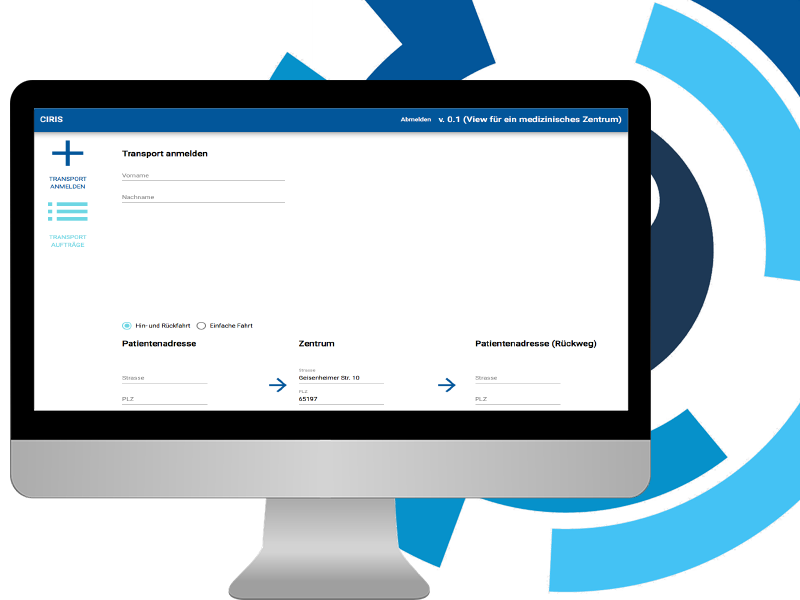
\includegraphics[width=\textwidth]{../Bilder/ciris.png}
	\captionof{figure}{Ciris: Eingabe von Transportfahrten}
	\label{img:ciris}
\end{minipage}
\end{center}
Potentielle Nutzer des Systems sind Patienten, medizinische Einrichtungen und Transportunternehmen, für die unterschiedliche Vorteile entstehen sollen:
\begin{itemize}
\item Für Patienten wird Folgendes geboten:
\begin{itemize}
\item Planung des Transports zum und vom Arzt/ Krankenhaus
\item Nutzung einer Smartphone App
\item Organisation von Serientransporten
\end{itemize}
\item Medizinische Einrichtungen können folgende Features nutzen:
\begin{itemize}
\item Transparente Transporte helfen beim Planen und Timing von Behandlungen.
\item Einfache Transportbestellung verringert Wartezeiten nach der Behandlung.
\item Automatisierte Erstellung von Transportscheinen
\end{itemize}
\item Für Transportunternehmen werden folgende Vorteile genannt:
\begin{itemize}
\item Strukturierte Routenplanung hilft bei der Verringerung von Wartezeiten und Leerfahrten.
\item Dynamische Neuplanung bei Änderungen oder Wegfallen von Fahrten verbessert die Effizienz.
\item Über Standortermittlung kann die gesamte Flotte überwacht werden.
\end{itemize}
\end{itemize}
Das generelle Ziel dieser Software deckt sich mit dem des Projekts, sie kann sich zu einem Konkurrenzprodukt entwickeln. Die Software hat jedoch noch nicht zeigen können, wie die Umsetzung dieses Konzepts aussehen soll.
\subsection{CareMan}
CareMan ist eine Softwarelösung für Einsatzdisposition, Dienstplanung, Finanzbuchhaltung und Fuhrparkmanagement der Firma „E/M/C Organisationsberatung und Datensysteme GmbH“ aus Kassel.
\begin{center}
\begin{minipage}{0.8\textwidth}
	\centering
	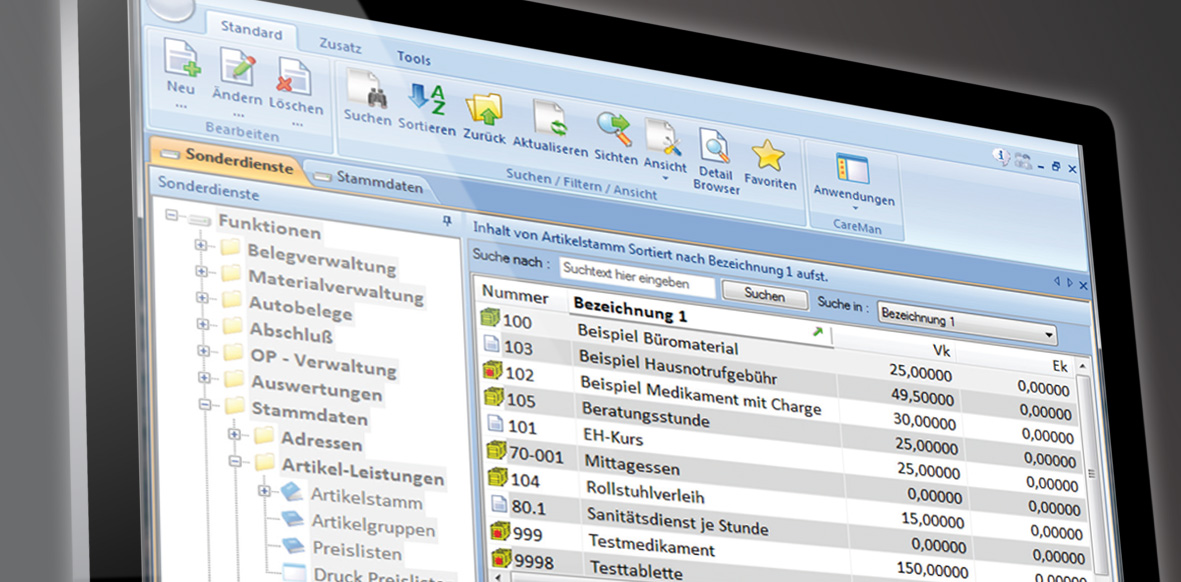
\includegraphics[width=\textwidth]{../Bilder/careman.jpg}
	\captionof{figure}{Reha-Transporte mit CareMan Office}
	\label{img:careman}
\end{minipage}
\end{center}
Das relevante Modul wird „CareMan Office“ genannt und als Branchensoftware für Rettungsdienste und Krankentransportunternehmen beworben. Sie ist also nur eine Software für Transportunternehmen und bietet keine Interaktion mit den Dienstleistungsnehmern an.
\begin{center}
\begin{tabular}{|p{0.45\textwidth}|p{0.45\textwidth}|}
\hline
\cellcolor{lightgray}\textbf{Vorteile}	&\cellcolor{lightgray}\textbf{Nachteile}\\
\hline
Einsatzabrechnung	&Keine Interaktion mit Dienstleistungsunternehmern\\
\hline
Routenoptimierung	&Keine unternehmensübergreifende Planung\\
\hline
Fuhrparkverwaltung	&\\
\hline
Vernetzte, mobile Anwendung für Fahrer	&\\
\hline
\end{tabular}
\end{center}
Als Planungssoftware für Transporte bietet diese Software viele Funktionen, ist jedoch als eine unternehmensübergreifende Lösung zur Vergabe von Krankentransportaufträgen nicht geeignet; auch weil es den externen Buchungsprozess nicht mit einbezieht.
\subsection{Recare}
„Recare“ ist eine Software für die Verteilung von Patienten auf Nachsorgeeinrichtungen und bezeichnet sich selbst als „führende digitale Entlassmanagement-Plattform“. Sie wird von der Berliner Firma „Recare Deutschland GmbH“ entwickelt.\\
\begin{center}
\begin{tabular}{|p{0.45\textwidth}|p{0.45\textwidth}|}
\hline
\cellcolor{lightgray}\textbf{Vorteile}	&\cellcolor{lightgray}\textbf{Nachteile}\\
\hline
Zentrale Vernetzung von Dienstleistungsanbietern und -nehmern	&Kein Transportmanagement\\
\hline
Automatische Vermittlung von Nachsorgeeinrichtungen	&\\
\hline
\end{tabular}
\end{center}
Auf das gegebene Problem bezogen kümmert sich diese Plattform allerdings nur um die Zielauswahl des Transports und nicht um den Transport selbst. Recare hat als Softwarelösung auch nicht den gleichen Fokus wie das zu konzipierende System. Jedoch ist die Art, mit der diese Software ihr Ziel erreichen will, fortschrittlich; das firmenübergreifende Netzwerk macht die zeitliche und organisatorische Abstimmung vieler unternehmensinternen Individuallösungen überflüssig.
\subsection{Fazit}
Auf dem Markt existieren ähnliche Systeme, deren Fokus sich an manchen Stellen mit dem des Projekts überschneidet. Das Produkt Ciris ist am ähnlichsten, konnte jedoch keine überzeugende Marktreife signalisieren. Durch diese Wettbewerbsanalyse kann jedoch viel Erfahrung für die Entwicklung einer passenden Lösung gewonnen werden.
\section{Sketching}
Nachdem wir die Anforderungen für unser Zielsystem festgelegt und die Konkurrenzprodukte analysiert hatten, vereinbarten wir die individuelle Erstellung von Papierprototypen. Beim nächsten Termin hatte jedes Teammitglied etwa fünf Minuten Zeit seine Umsetzung den anderen vorzustellen. Danach gab es jeweils eine kurze Feedbackrunde, in welcher die positiven und negativen Aspekte der Umsetzung diskutiert wurden. Wir einigten uns schließlich auf gemeinsame Lösungsvorstellungen und überarbeiteten unsere Prototypen in einer zweiten Iteration. Die Änderungen wurden im Anschluss daran erneut für jeweils fünf Minuten diskutiert. Nach der zweiten Iteration skizzieren wir einen gemeinsamen Lösungsansatz in draw.io. Dieser diente später als Grundlage für die finale Umsetzung in Axure.
\subsection{Papierprototyp – Florian Klamer}
\begin{center}
\begin{minipage}[b]{0.7\textwidth}
	\centering
	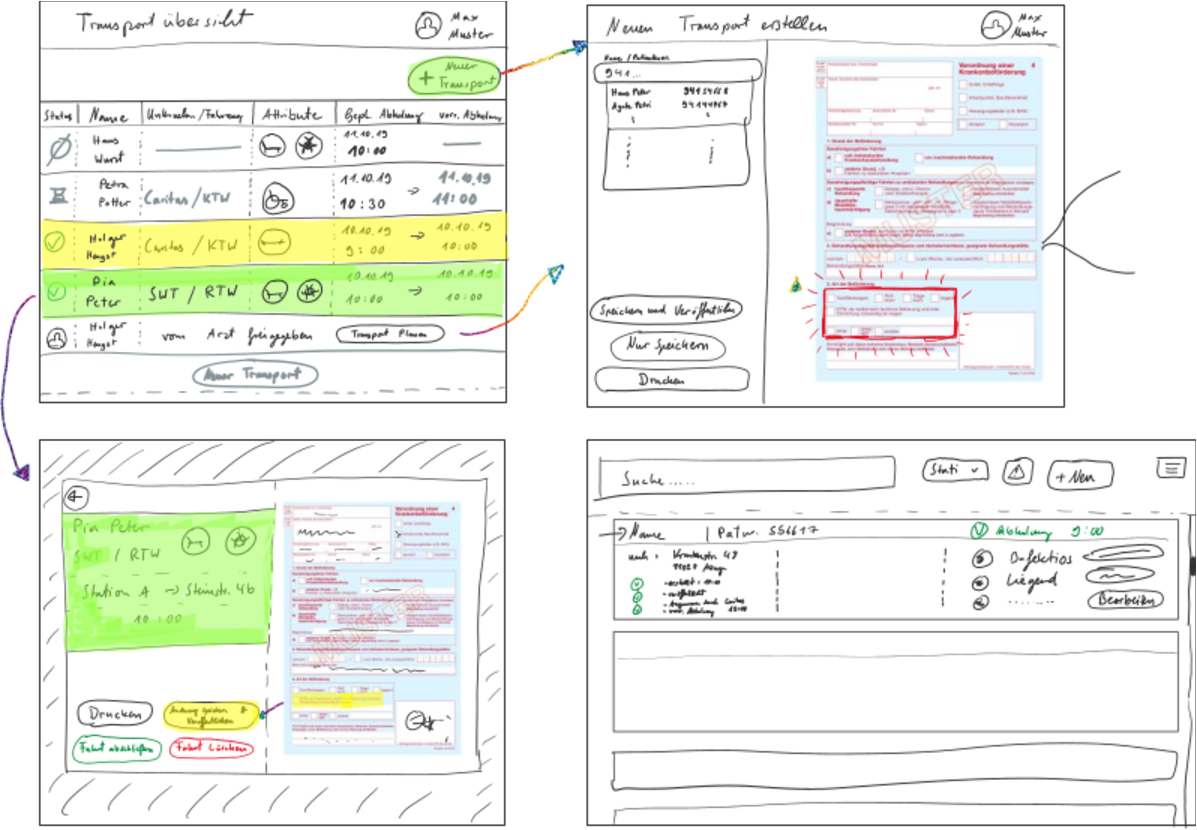
\includegraphics[width=\textwidth]{../Bilder/prototypFlo.pdf}
	\captionof{figure}{Prototyp Klamer}
	\label{img:klamer}
\end{minipage}
\end{center}
\subsection{Papierprototyp – Felix Richter}
\begin{center}
\begin{minipage}[b]{0.7\textwidth}
	\centering
	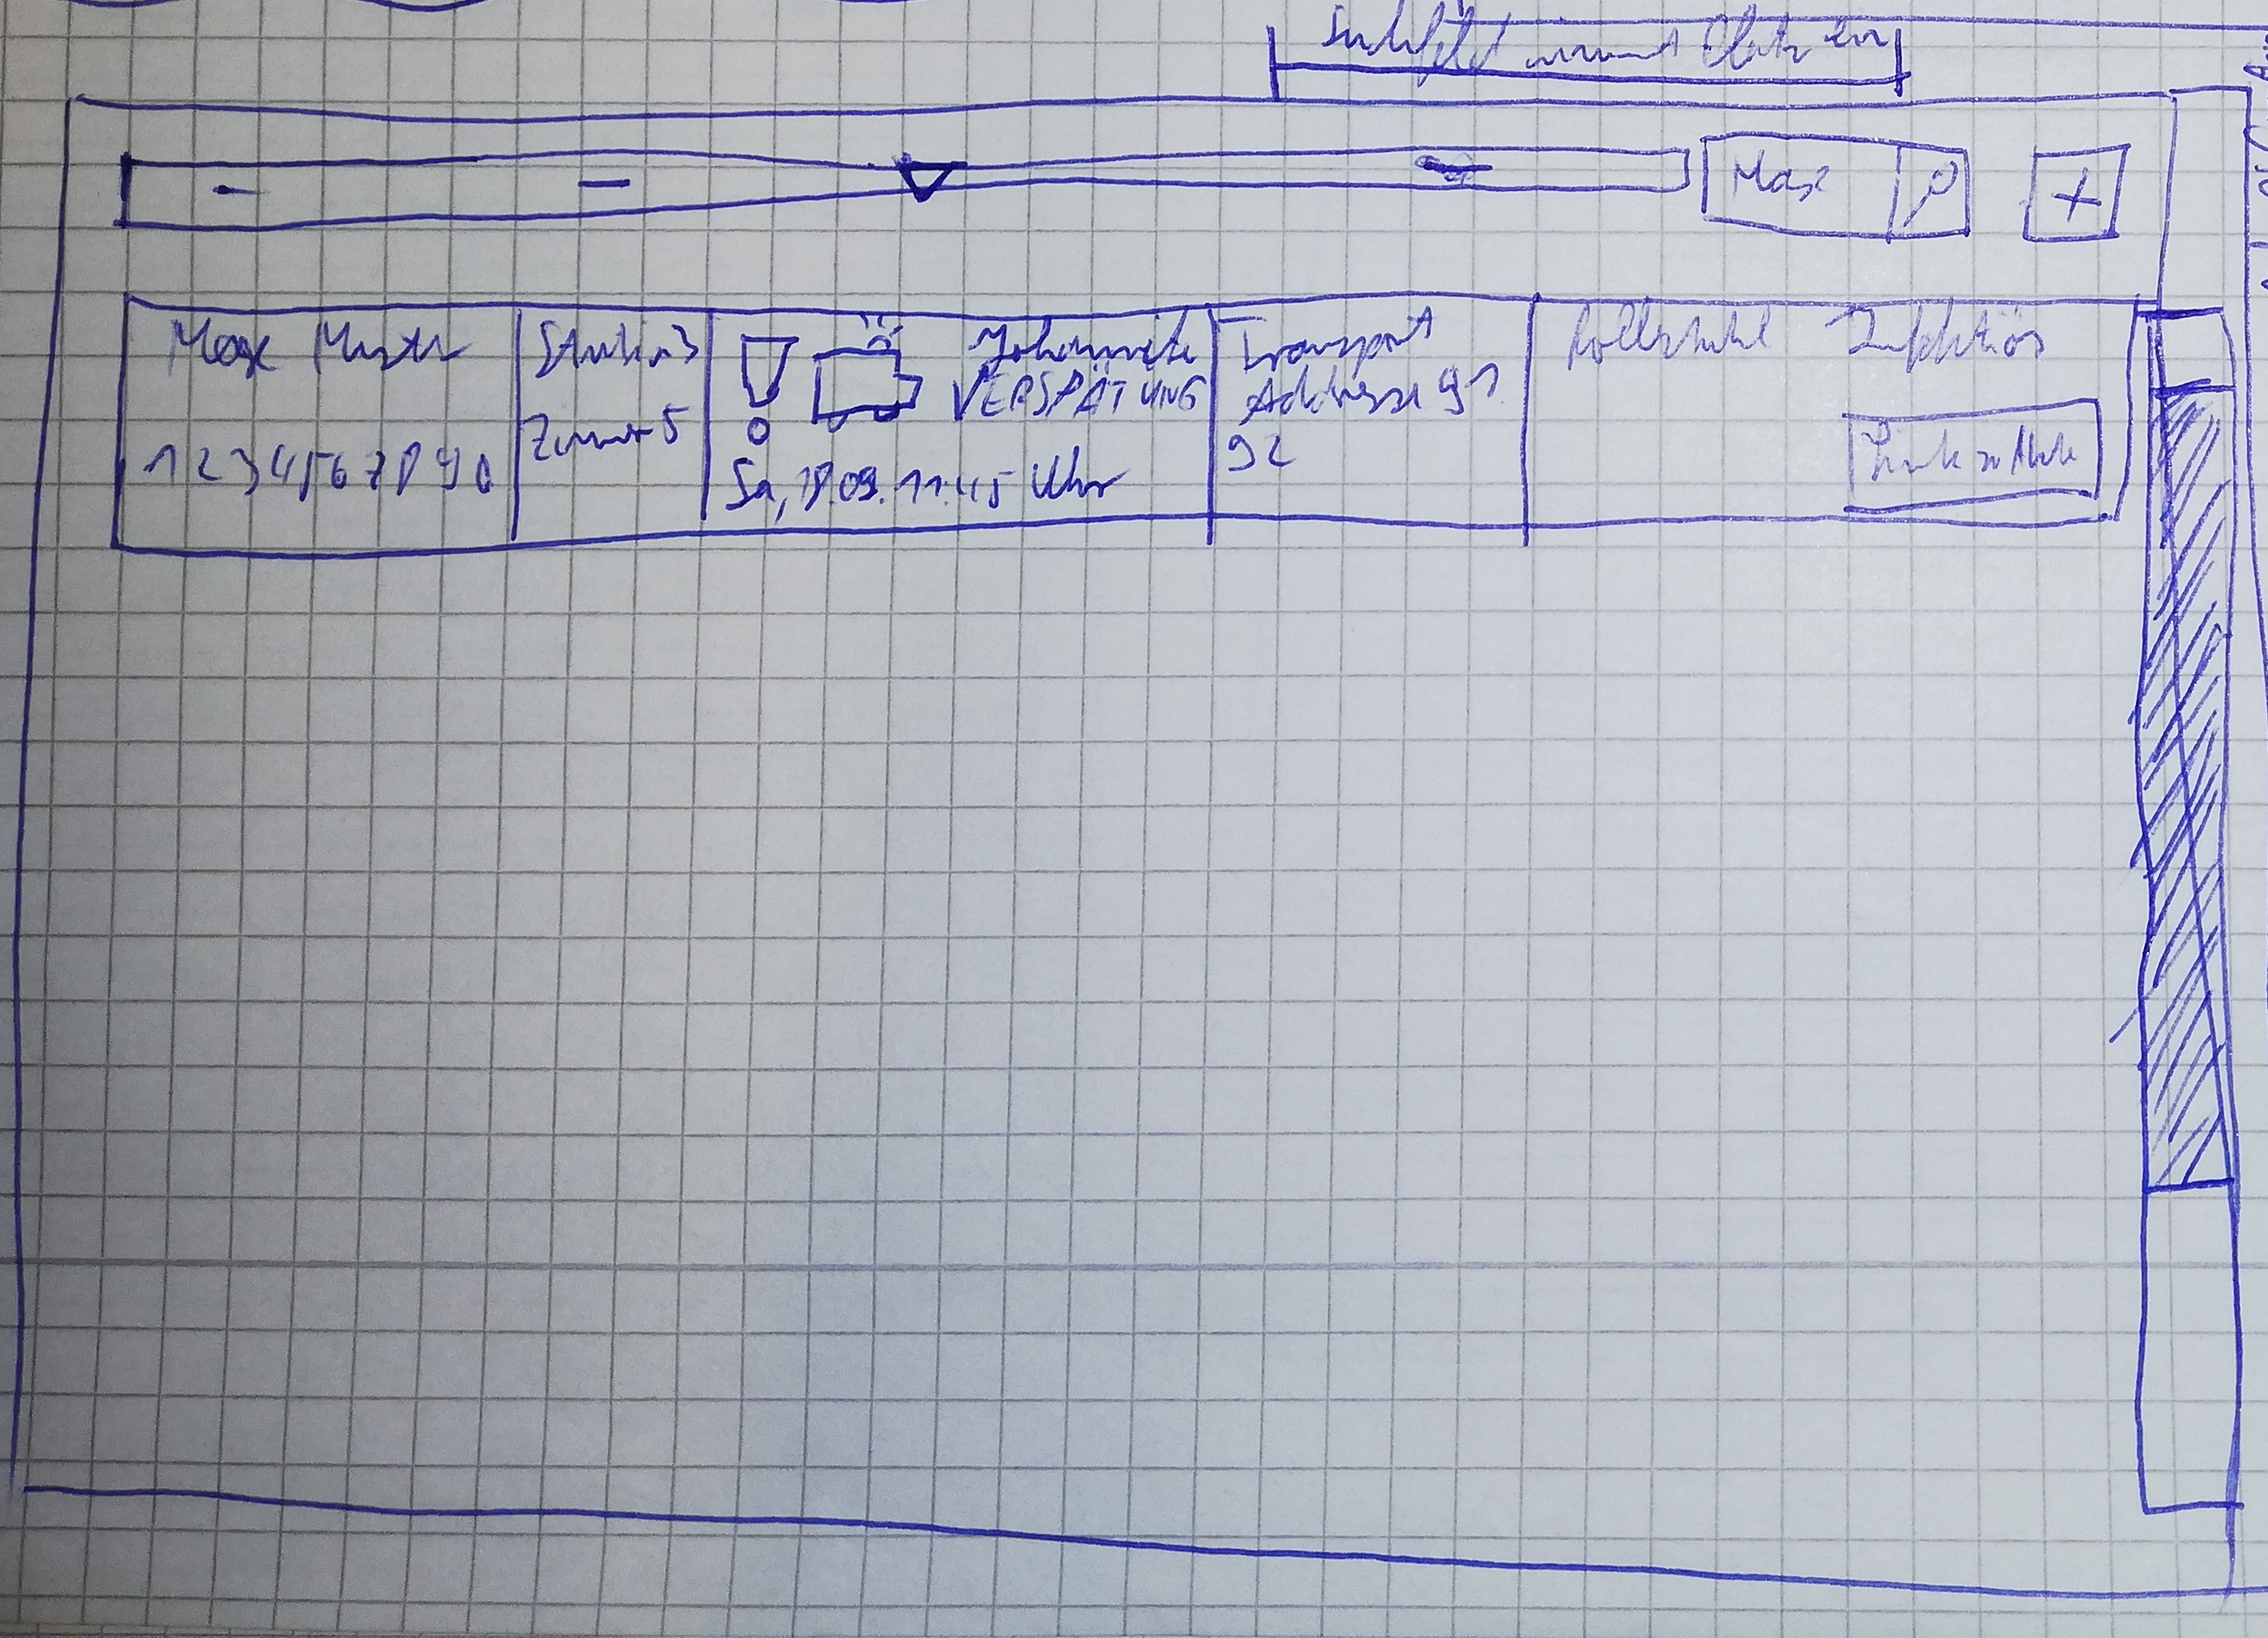
\includegraphics[width=\textwidth]{../Bilder/uebersicht.jpg}
	\captionof{figure}{Prototyp Richter 1}
	\label{img:richter1}
\end{minipage}
\end{center}
Der Arzt oder die Schwester muss sich zuerst einloggen. Die darauffolgende Ansicht ist für beide die gleiche, aber der Arzt hat die Möglichkeit Patienten mit Hilfe des Plus-Buttons zu entlassen. In Boxen werden die wichtigsten Informationen aller Patienten angezeigt, die entlassen werden sollen. Stammdaten, Zimmernummer und Besonderheiten, wie z.B. „Rollstuhlfahrer“ oder „Infektiös“, werden immer dargestellt, während aktuelle Informationen zum Transport nur angezeigt werden, wenn dieser schon angefordert, bzw. angenommen wurde. In den Boxen sind kleine Links zum schnellen Öffnen der Patientenakte. Um in diesen Patienten zu suchen, bzw. diese zu sortieren wird die gleiche Ansicht verwendet.\\
\begin{center}
\begin{minipage}[b]{0.8\textwidth}
	\centering
	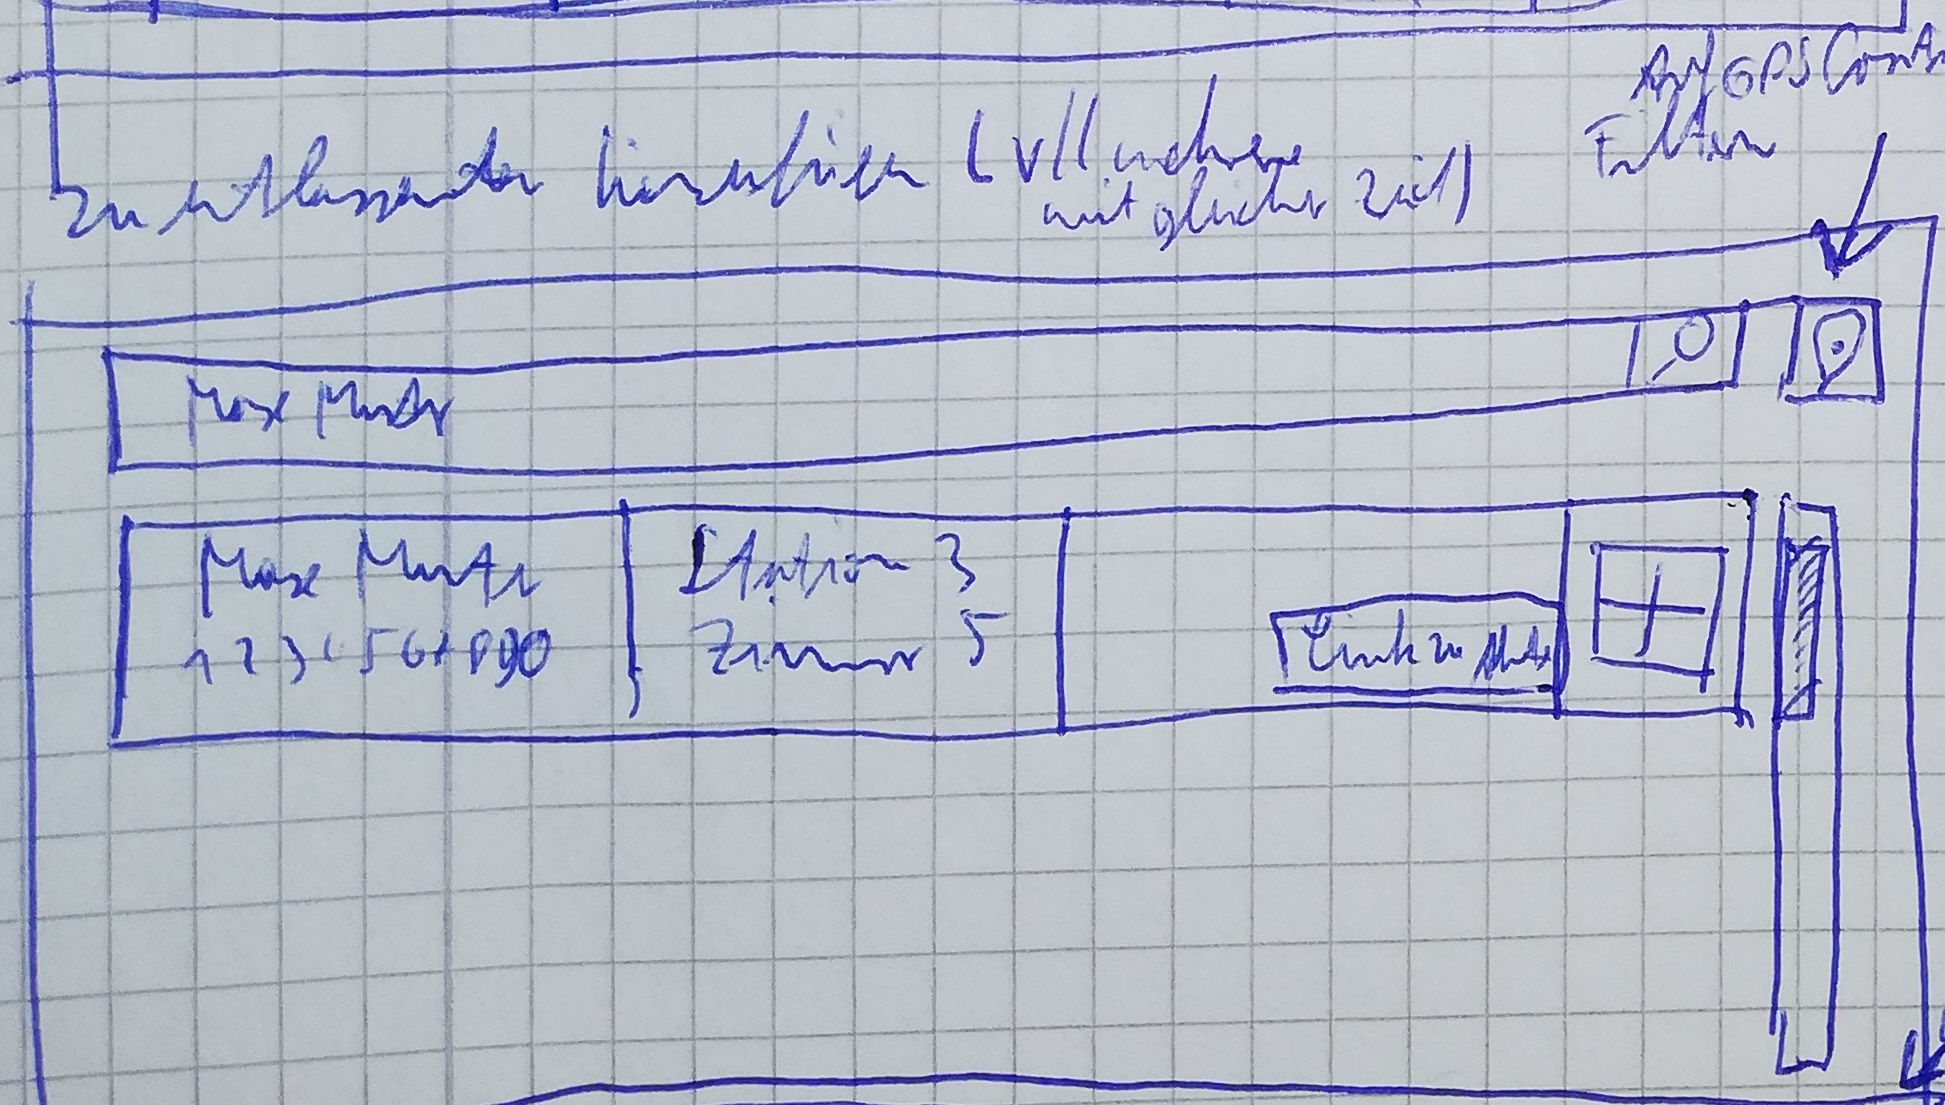
\includegraphics[width=\textwidth]{../Bilder/hinzufuegen.jpg}
	\captionof{figure}{Prototyp Richter 2}
	\label{img:richter2}
\end{minipage}
\end{center}
Die Ansicht zum Entlassen von Patienten ist eine verkleinerte Variante der vorherigen mit nur Stammdaten. Patienten können über eine Suche gefunden werden. Weil die Applikation auch auf Smartphones funktioniert, kann der Arzt, wenn er im Zimmer des Patienten ist, über die aktuelle Position nach ihm suchen.\\[1.5em]
\begin{minipage}{0.4\textwidth}
	\centering
	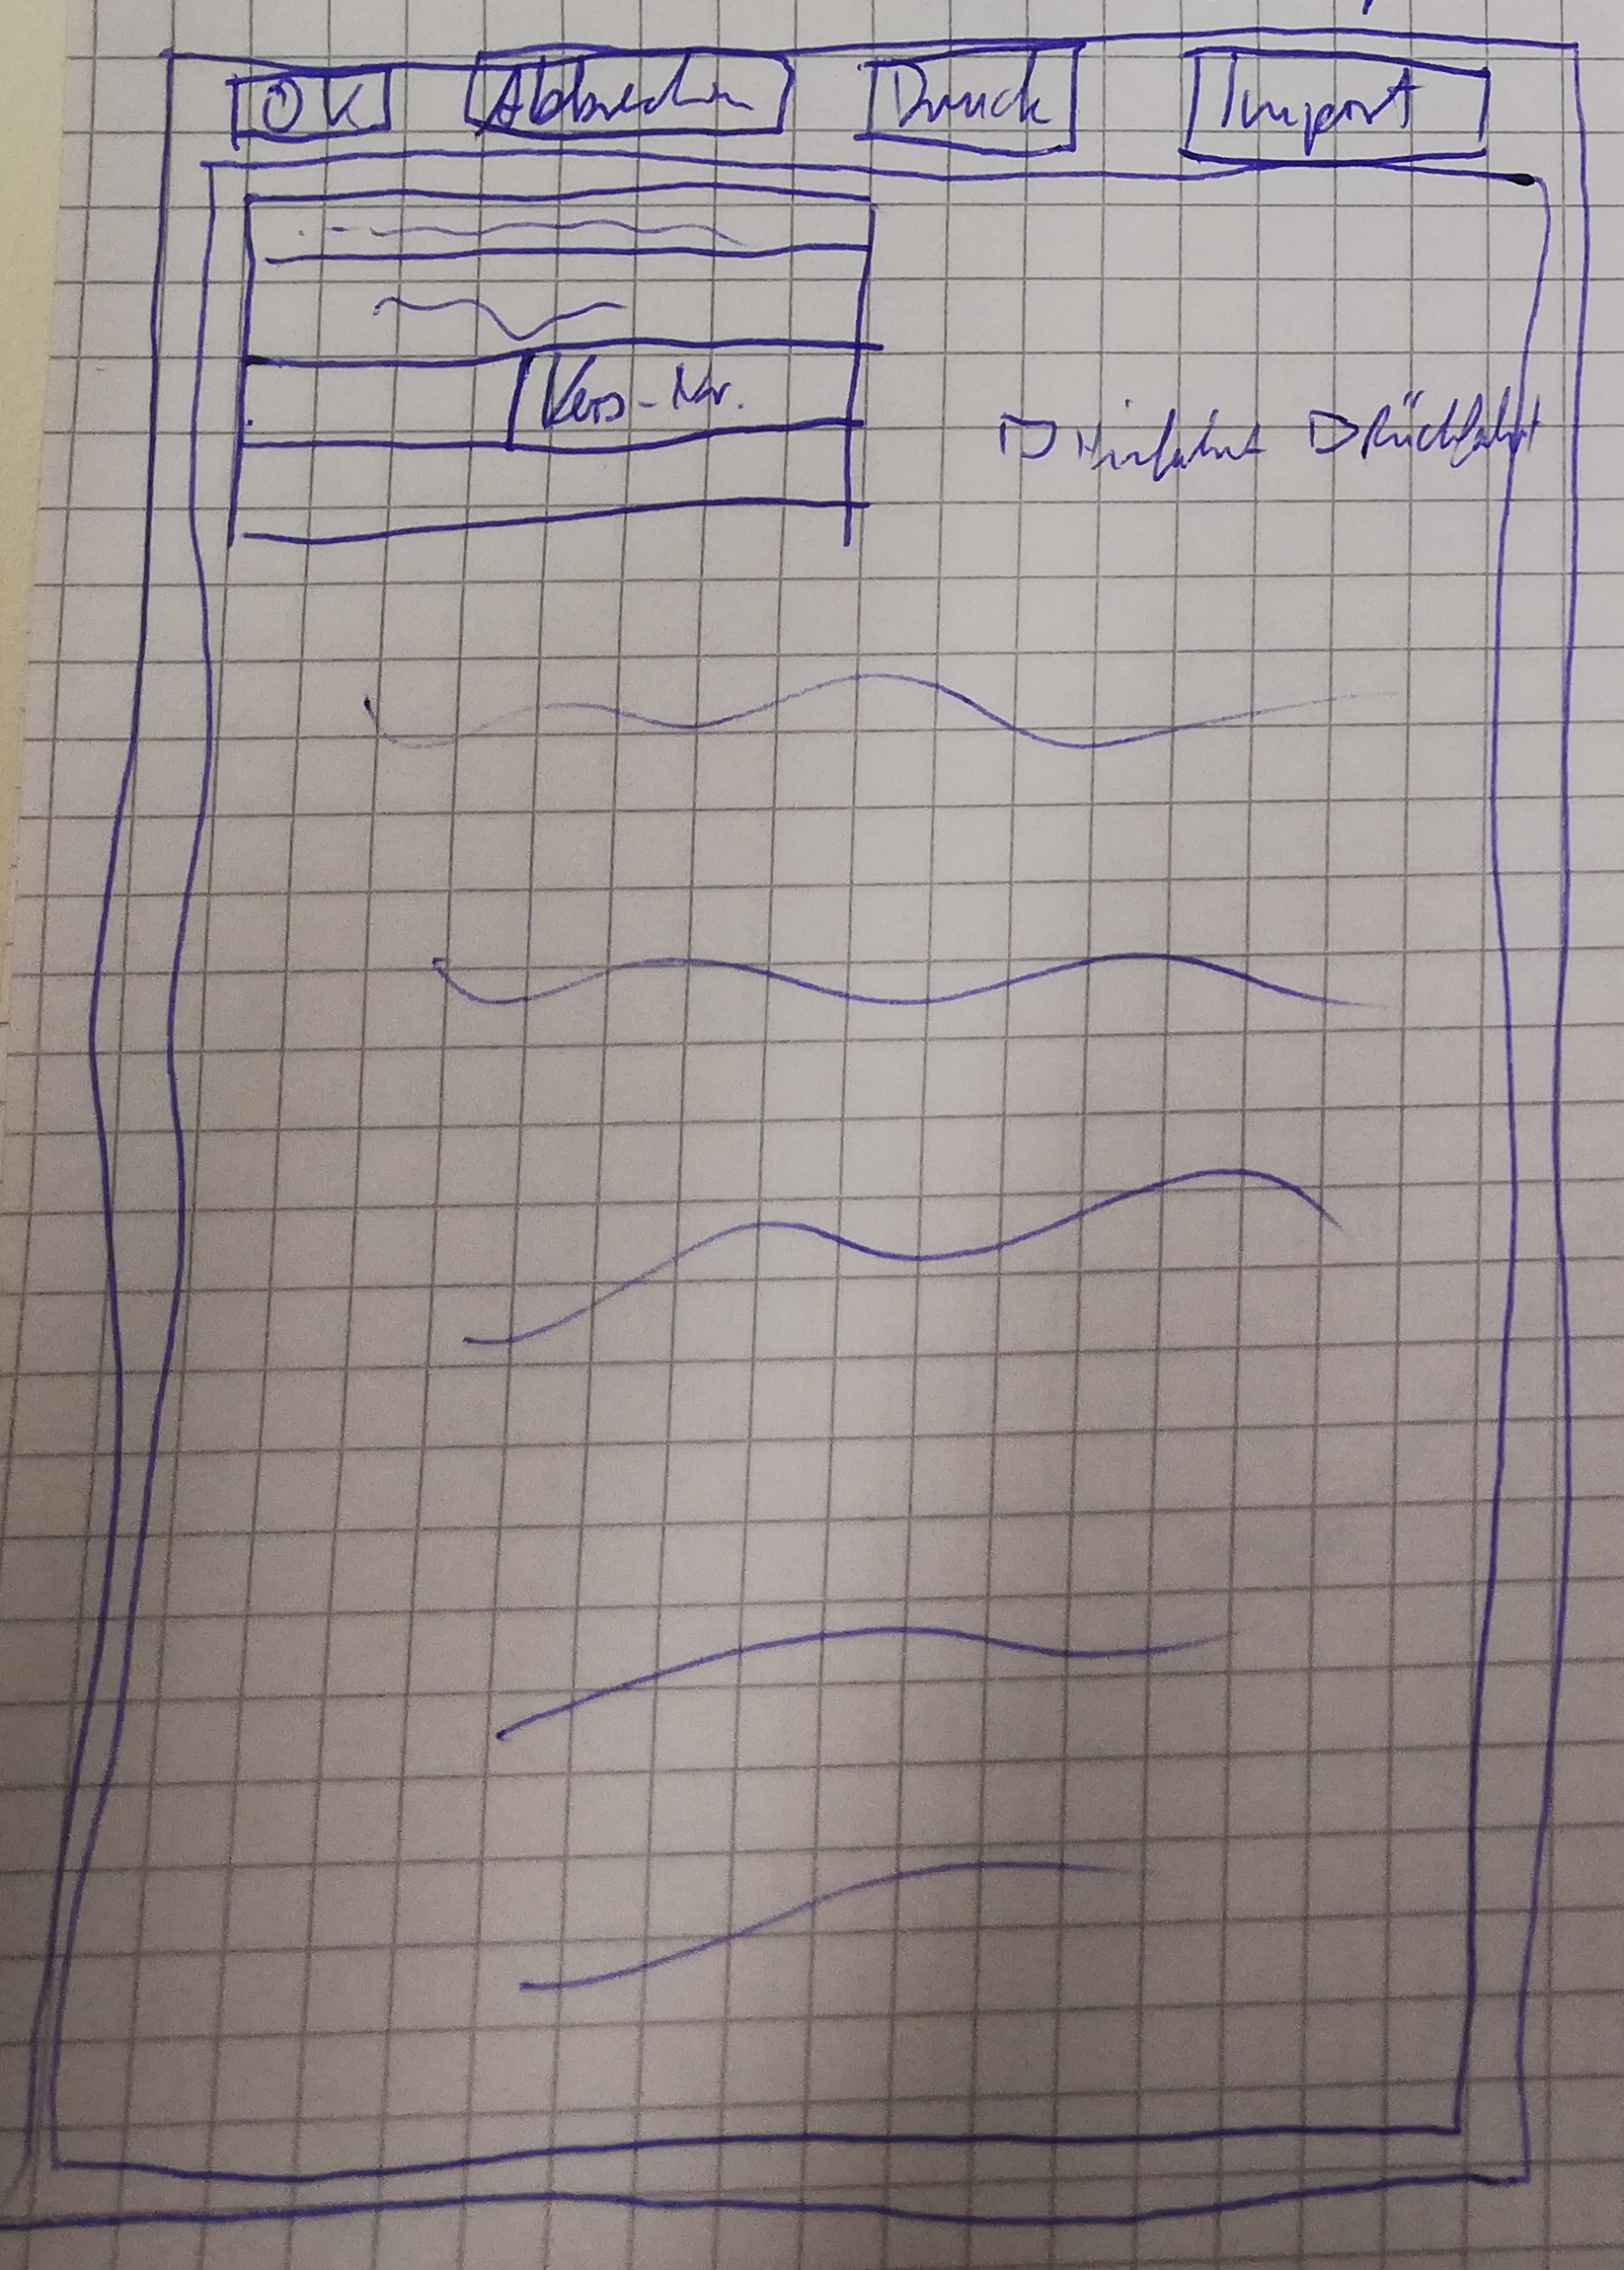
\includegraphics[width=\textwidth]{../Bilder/flaxxy.jpg}
	\captionof{figure}{Prototyp Richter 3}
	\label{img:richter2}
\end{minipage}
\hspace{0.05\textwidth}
\begin{minipage}{0.55\textwidth}
Auf die einzelnen Boxen der Übersicht kann geklickt werden. Diese Detailansicht wird darauf hin geöffnet. Sie entspricht dem Patientenbeförderungsschein. Die einzelnen Felder können bearbeitet werden; Daten können aber auch von der Patientenakte importiert werden. Ein Button zum Drucken steht hier auch bereit.\vspace{5cm}\\
\end{minipage}
\subsection{Papierprototyp – Thomas Zenger}
\begin{center}
\begin{minipage}[b]{0.48\textwidth}
	\centering
	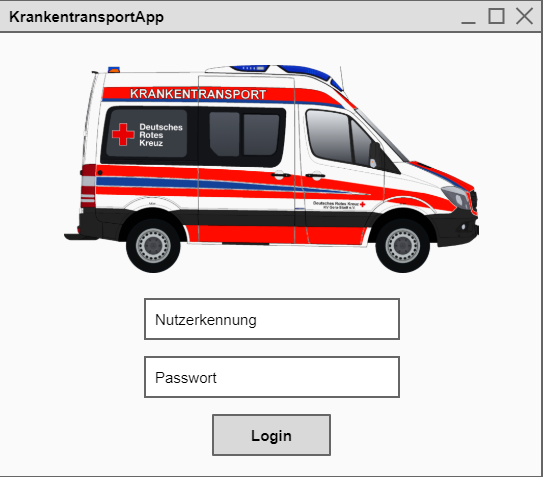
\includegraphics[width=\textwidth]{../Bilder/loginpage.png}
	\captionof{figure}{Prototyp Zenger 1}
	\label{img:zenger1}
\end{minipage}
\begin{minipage}[b]{0.48\textwidth}
	\centering
	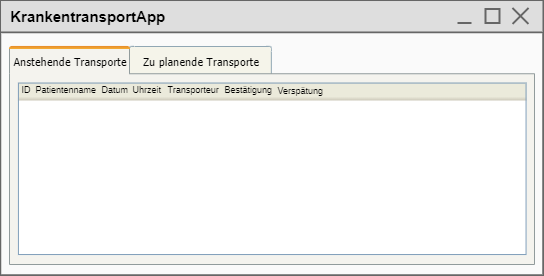
\includegraphics[width=\textwidth]{../Bilder/mainpage.png}
	\captionof{figure}{Prototyp Zenger 2}
	\label{img:zenger2}
\end{minipage}
\end{center}
\begin{center}
\begin{minipage}[b]{0.48\textwidth}
	\centering
	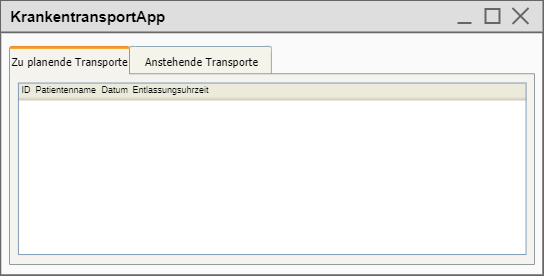
\includegraphics[width=\textwidth]{../Bilder/mainpage_1.png}
	\captionof{figure}{Prototyp Zenger 3}
	\label{img:zenger3}
\end{minipage}
\begin{minipage}[b]{0.48\textwidth}
	\centering
	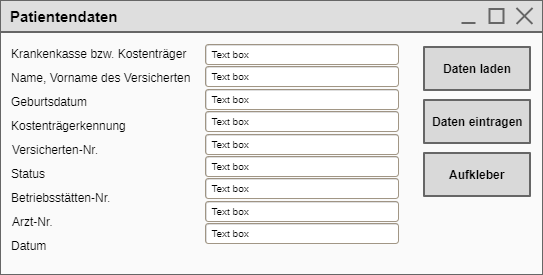
\includegraphics[width=\textwidth]{../Bilder/verordnungpage.png}
	\captionof{figure}{Prototyp Zenger 4}
	\label{img:zenger4}
\end{minipage}
\end{center}
Beim Start des Programmes wird eine einfache Login In Maske zur Anmeldung aufgerufen. Im Zuge eines Single Sign-on Systems kann auf den extra Login verzichtet werden.\\
Die Hauptansicht des Programms wird übersichtlich und einfach gehalten. Im wesentlichen besteht die Ansicht aus zwei Tabs. Der erste Tab listet alle anstehenden (d.h. bereits geplante) Transporte auf. Im zweiten Tab werden Patienten aufgelistet, für die noch ein Transport zu planen ist.\\
Mit einem Doppelklick auf einen Listeneintrag öffnet man die 2. Ansicht. Die Ansicht beinhaltet eine Maske zur Bearbeitung der Patienten- und Transportdaten. Drei Buttons beinhalten die Funktionalität des Programms. Daten können aus der Patientenakte geladen werden. Sind alle Daten erfasst können diese per ``Daten eintragen'' gespeichert und der Transport übermittelt werden. Der Aufkleber für den Schein ``Verordnung Krankentransport'' kann per Knopfdruck ausgedruckt werden.
\subsection{Papierprototyp – Tobias Winter}
\begin{center}
\begin{minipage}[b]{0.48\textwidth}
	\centering
	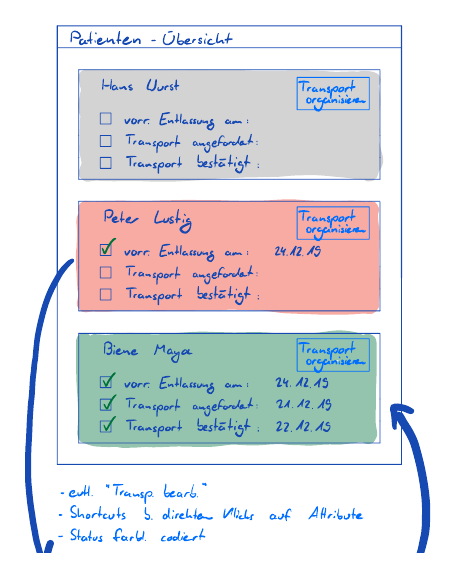
\includegraphics[width=\textwidth]{../Bilder/PrototypTobias1.png}
	\captionof{figure}{Prototyp Winter 1}
	\label{img:winter1}
\end{minipage}
\begin{minipage}[b]{0.48\textwidth}
	\centering
	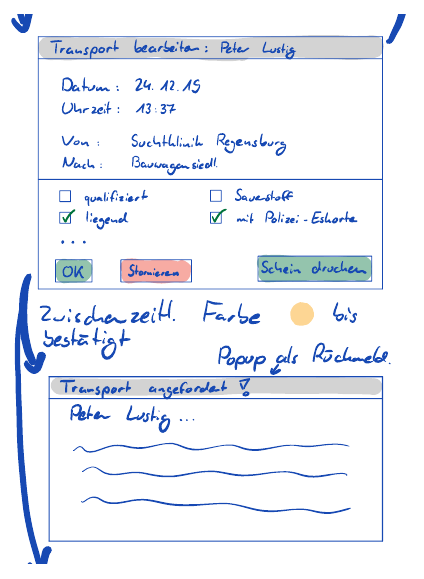
\includegraphics[width=\textwidth]{../Bilder/PrototypTobias2.png}
	\captionof{figure}{Prototyp Winter 2}
	\label{img:winter2}
\end{minipage}
\end{center}
\begin{center}
\begin{minipage}{0.5\textwidth}
	\centering
	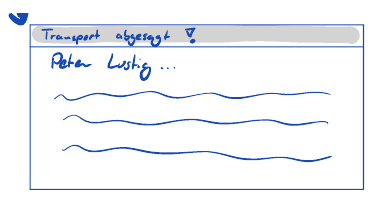
\includegraphics[width=\textwidth]{../Bilder/PrototypTobias3.png}
	\captionof{figure}{Prototyp Winter 3}
	\label{img:winter3}
\end{minipage}
\end{center}
Der digitale Papierprototyp verfolgt im Wesentlichen zwei Grundideen: Äußerste Einfachheit der Oberfläche sowie extensive Nutzung farblicher Kodierung.\\

Die Einfachheit des Interfaces ist auf mehreren Ebenen wichtig. Zum einen wird dadurch die Darstellung auf Mobilgeräten vereinfacht bzw. überhaupt erst ermöglicht, zum anderen soll das System auch unter Zeitdruck oder im Nachtdienst bei erhöhter Müdigkeit einfach bedient werden können und dadurch sowohl zur Benutzung einladen, als auch Fehler vermeiden.\\

Demselben Grundgedanken folgt die farbliche Kodierung. Einerseits ist so der Stand der jeweiligen Transporte auch bei nur flüchtigem Blick sofort zu erkennen, zum anderen kann dadurch Platz eingespart werden, der z.B. für die textuelle Beschreibung der farblichen Kodierung aufgewendet hätte werden müssen.\\
 
Der komplette Vorgang wird in der Stati unterteilt: vorraussichtliche Entlassung bekannt, Transport angefordert und Transport bestätigt. Bearbeitung einer Patientenkarte ist durch Klick auf diese, oder durch Klick auf “Transport organisieren” möglich. Der Button wurde eingefügt, da es u.U. nicht jedem Anwender einleuchtet, dass ein einfacher Klick auf die Karte zur Bearbeitung führt.

\subsection{Papierprototyp – Sebastian Brunner}
\begin{minipage}{\textwidth}
	\centering
	\includesvg[width=\textwidth]{../Bilder/PrototypeBrunner.svg}
	\captionof{figure}{Prototyp Brunner}
	\label{img:brunner}
\end{minipage}\\[0.5em]
\subsubsection*{Startseite:}
Die Startseite meines Papierprototypen zeigt zunächst nur die wichtigsten Transporte (z.B. innerhalb der nächsten Stunde). Transporte, die weiter in der Zukunft liegen und damit für den Nutzer weniger relevant sind bleiben eingeklappt. Bei Bedarf kann jeder Transport individuell auf- und wieder eingeklappt werden.
\subsubsection*{Patienten - Karte:}
Ein eingeklappter Transport zeigt nur den Patientennamen, zur eindeutigen Identifizierung die Patientennummer sowie den aktuellen Status des Transports (übermittelt, bestätigt, storniert). Dies genügt, um einen Patiententransport manuell oder später über die Suchleiste aufzufinden. Im ausgeklappten Zustand wird zusätzlich das Transportdatum und -ziel angezeigt. Darunter befindet sich eine kurze Übersicht der bereits abgeschlossenen und noch aussehenden Ereignisse (z.B. Transport übermittelt, Transport angenommen / storniert). Die wichtigsten Informationen des Patiententransports werden zudem mit Piktogrammen und einem kurzen Text visualisiert.
\subsubsection*{Kopfzeile:}
Neben einer Suchfunktion für eingetragene Patiententransporte bietet die Kopfzeile eine Benachrichtigungsfunktion, welche Auskunft über Statusänderungen bei Patiententransporten gibt (z.B. TransportXY wurde angenommen / storniert). Neue Transporte können ebenso über einen Button in der Kopfzeile erstellt werden.
\subsubsection*{Neuer Transport, Patientensuche und Transportschein:}
Um einen neuen Transport zu erstellen muss zunächst der zu entlassene Patient ausgewählt werden. Die Daten stammen dabei aus der Patientendatenbank des Krankenhauses. Um den zu entlassenen Patienten schnell aufzufinden wird hier, wie bereits bei den Transporten, eine Suche nach Patientenname oder -nummer angeboten.\\

Beim Klick auf „Entlassung“ werden die personenbezogenen Daten des Patienten aus der elektronischen Patientenakte in den Transportschein übernommen. Nun kann der Nutzer die restlichen Inhalte des Transportschein ausfüllen, die relevanten Inhalte an den Transportdienstleister übermitteln und den Transportschein drucken. Der Transport wird gespeichert und anschließend auf der Startseite angezeigt. Jeder Transport kann nachträglich bearbeitet oder wieder storniert werden.
\section{Axure Prototyp}
Ansprechende Designvorlagen sind in Axure RP 9 leider meist kostenpflichtig. Daher haben wir uns entschlossen unseren Axure Prototypen auf Basis des zuvor mit draw.io skizzieren Prototyps umzusetzen. Wir mussten in Axure neben der Navigationszeile somit nur noch die Klick-, Such- und Datenhaltungsfunktionen implementieren.
\subsection{gemeinsamer Axure Prototyp}
\subsubsection{Startseite}
\begin{center}
\begin{minipage}{0.8\textwidth}
	\centering
	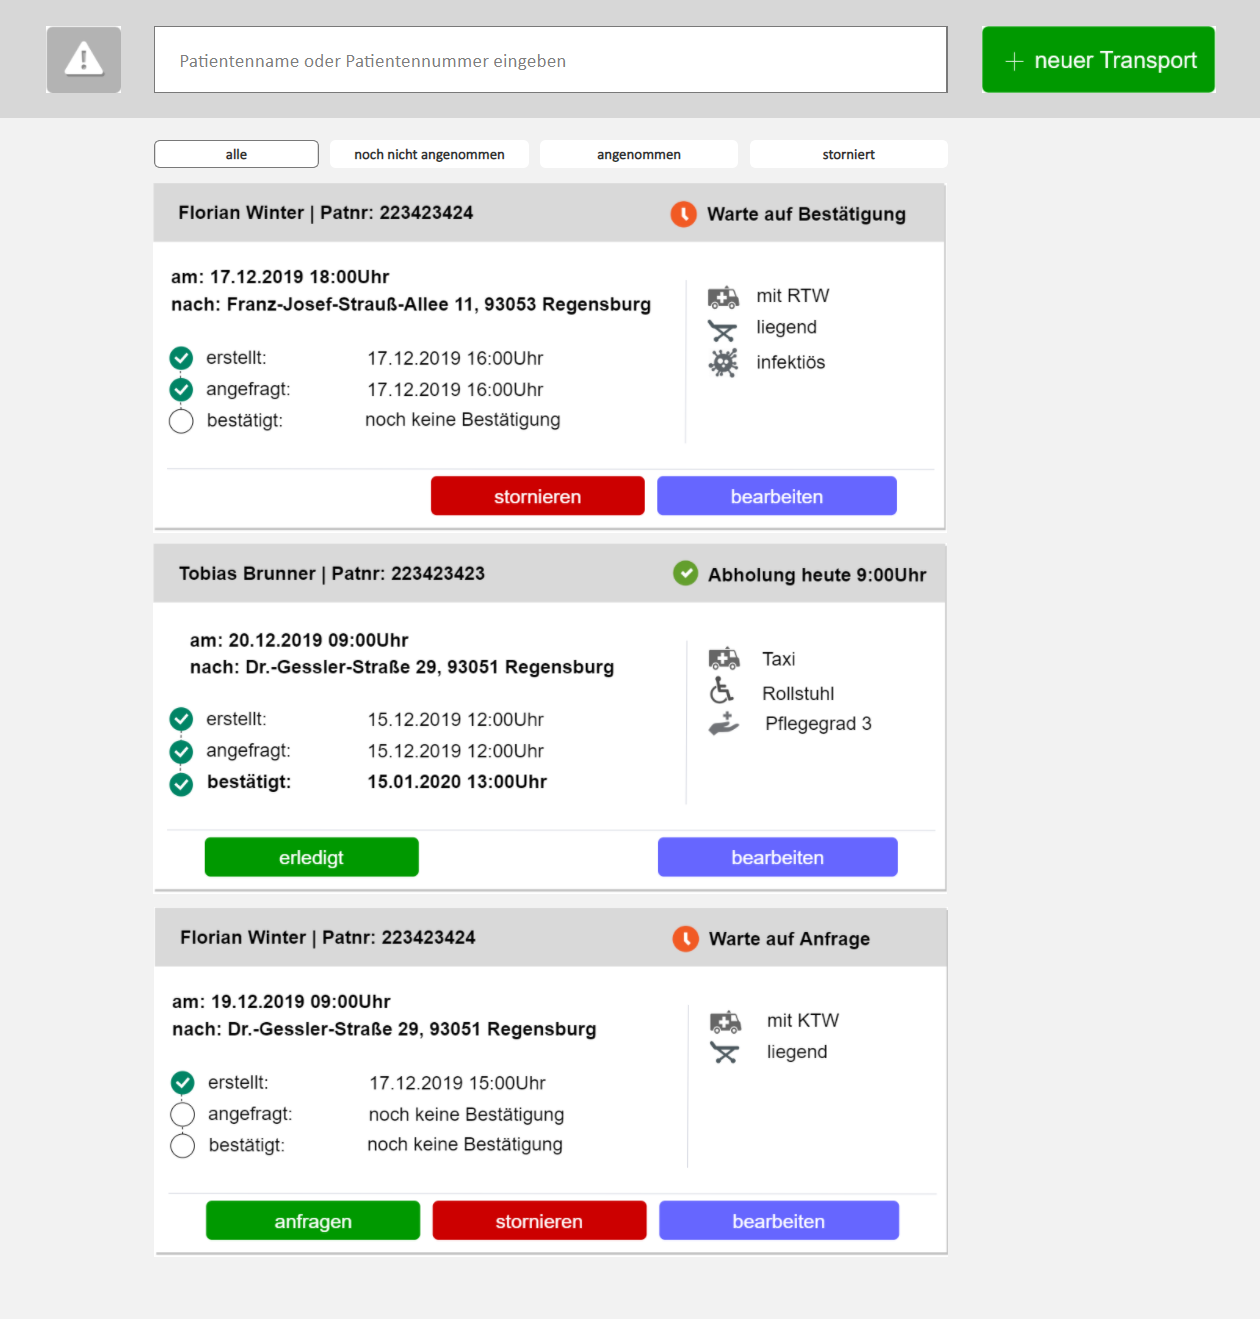
\includegraphics[width=\textwidth]{../Bilder/ap1Startseite.png}
	\captionof{figure}{Axure - Startseite (Alle Transporte)}
	\label{img:ap1start}
\end{minipage}
\end{center}
Die Startseite unseres Axure Prototypen zeigt zunächst alle eingetragenen Patiententransporte sortiert nach dem frühesten Abholdatum. Die angezeigten Transporte können über die Suche und der Navigationsleiste eingegrenzt werden. Neue Transporte können ebenfalls über die Startseite eingetragen werden.
\subsubsection{Navigationsleiste}
\begin{center}
\begin{minipage}{0.8\textwidth}
	\centering
	
\includegraphics[width=\textwidth]{../Bilder/ap1Nav.png}
	\captionof{figure}{Axure - Navigationsleiste}
	\label{img:ap1nav}
\end{minipage}
\end{center}
Um die Transportübersicht für verschiedene Anwendungsfälle anzupassen haben wir die Transporte in unterschiedliche Kategorien / Reiter unterteilt:\\
\begin{itemize}
\item Beim Start unseres Prototypens ist Reiter „alle“ vorausgewählt, dieser zeigt alle Patiententransporte unabhängig von deren aktuellen Status.
\item Im Reiter „noch nicht angenommen“ befinden sich Transporte, welche bisher nur erstellt oder vom Fuhrpark noch nicht angenommen wurden. Es kommt z.B. vor, dass die Entlassung eines Patienten in der morgendlichen Besprechung angeordnet wird, jedoch zu diesem Zeitpunkt noch nicht alle relevanten Details für den Transport festsehen. Das Pflegepersonal kann später in diesem Reiter alle Transporte mit noch fehlenden Details einsehen und fertig planen. 
\item Der Reiter „angenommen“ zeigt nur vom Fuhrpark bestätigte Transporte an. Diese Ansicht ist hilfreich, um einzusehen welche Patienten demnächst abgeholt werden und ggfs. für den Transport schon einmal vorbereitet werden können (Rollstuhl, Sauerstoff, etc…). 
\item Im Reiter „storniert“ werden Transporte angezeigt, die vom Fuhrpark zunächst angenommen wurden, jedoch beispielsweise aus zeitlichen Gründen wieder storniert werden mussten. Stornierte Transporte sind meist mit einem zeitlichen Mehraufwand verbunden und können deshalb gesondert angezeigt werden.
\end{itemize}
\subsubsection{Patiententransport - Karte}
\begin{center}
\begin{minipage}{0.8\textwidth}
	\centering
	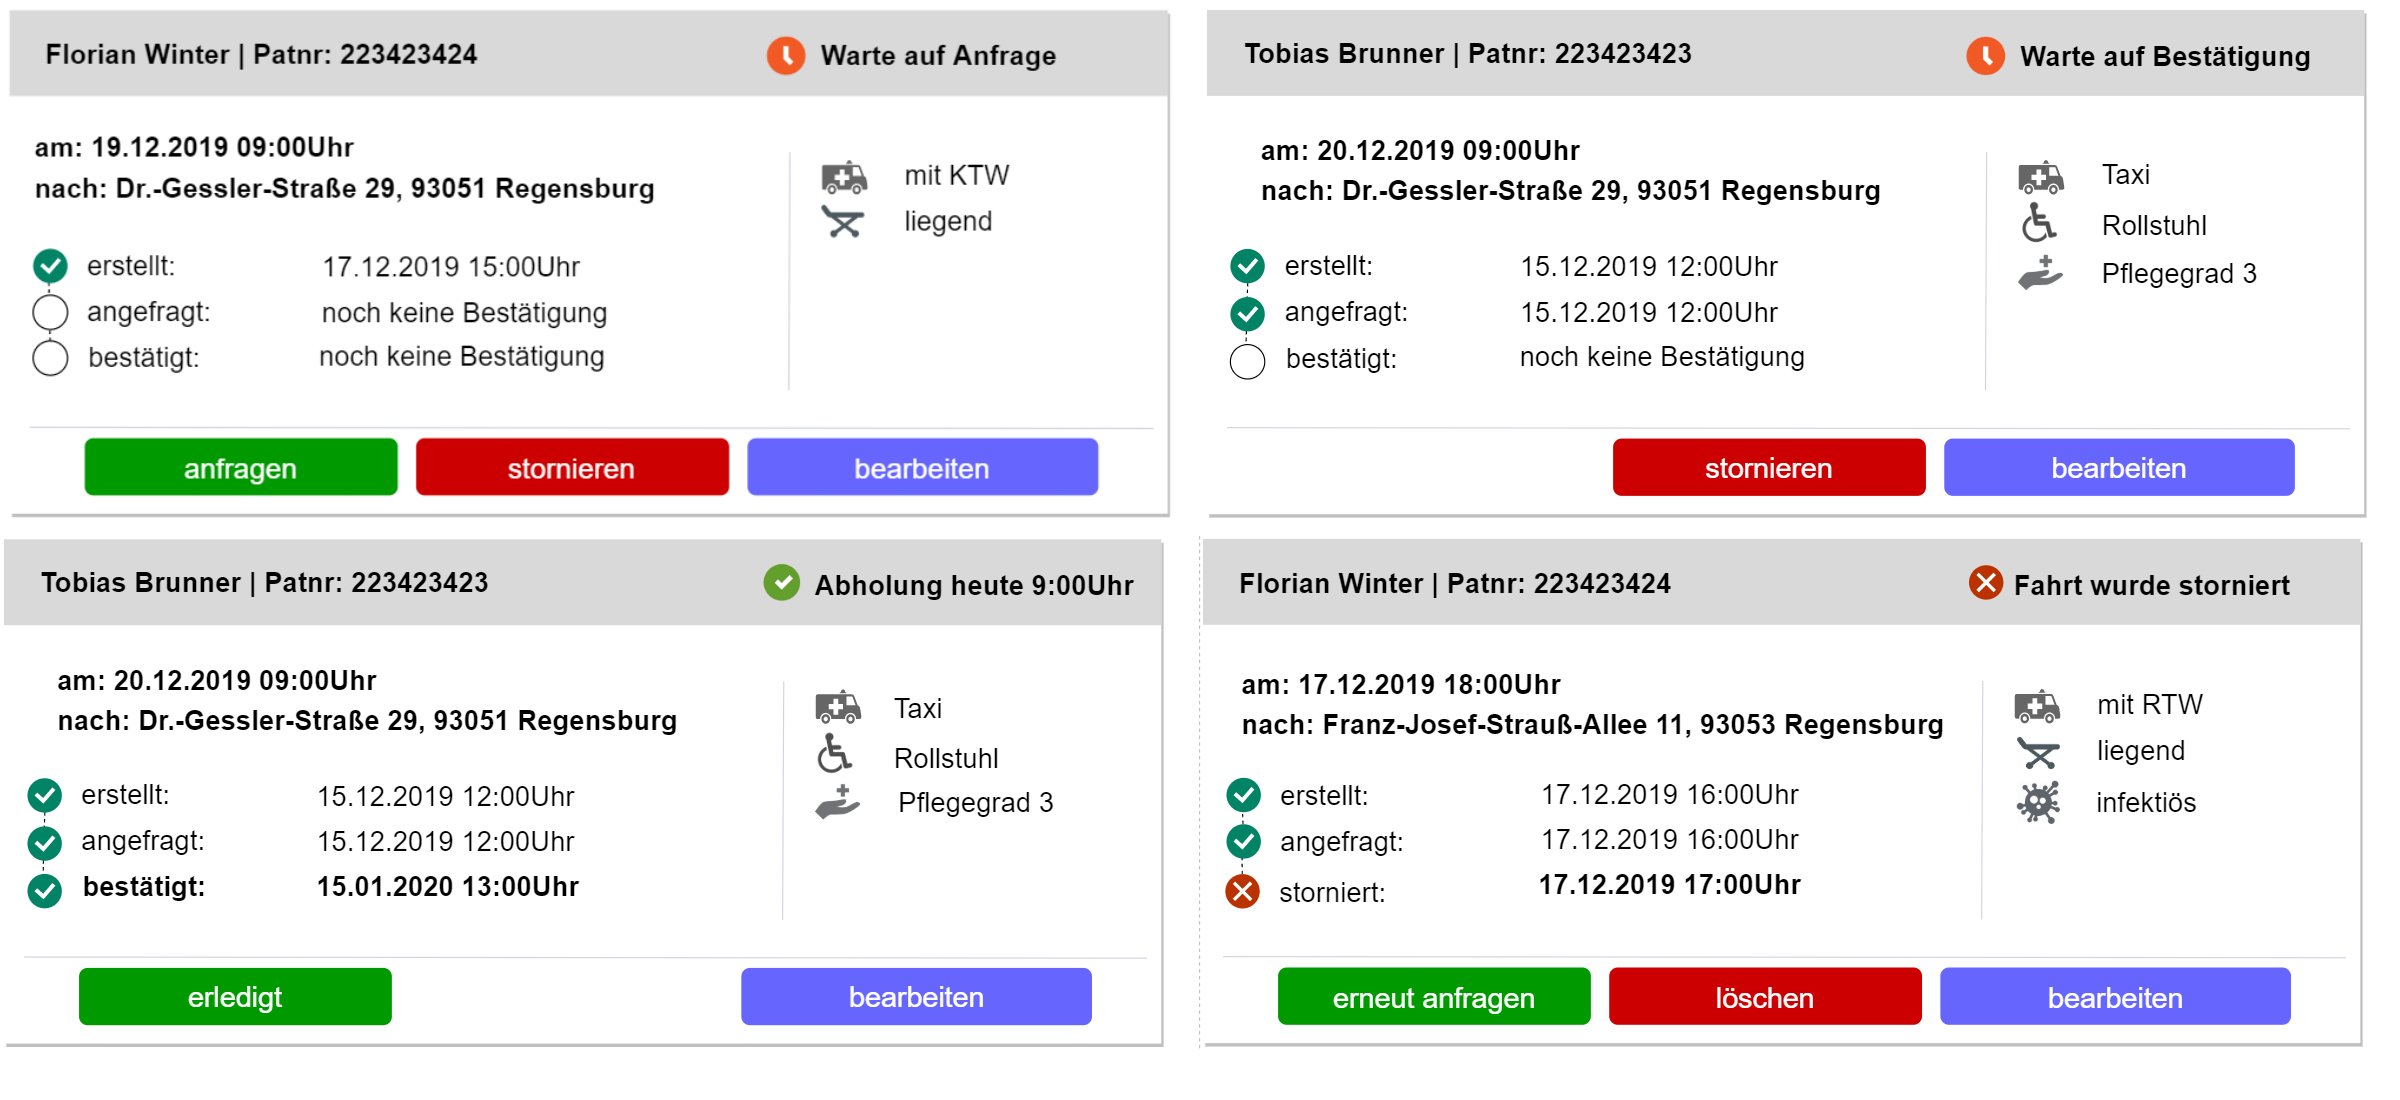
\includegraphics[width=\textwidth]{../Bilder/ap1Card.png}
	\captionof{figure}{Axure - Patiententransport-Karte}
	\label{img:ap1card}
\end{minipage}
\end{center}
Identifizierung die Patientennummer sowie den aktuellen Status des Transports an. Darunter befindet sich der Transporttermin und -ort, sowie eine kurze Übersicht der bereits abgeschlossenen und noch aussehenden Ereignisse des Patiententransports (erstellt, angefragt, bestätigt, storniert).\\
\begin{itemize}
\item Der Punkt „erstellt“ ist abgehakt, sobald ein Transport eingetragen wird.
\item Wenn alle Details des Transports geklärt sind, kann dieser fertig geplant und beim Fuhrpark „angefragt“ werden.
\item Der Fuhrpark hat nun die Möglichkeit den Transport zu bestätigen („bestätigt“) und diesen später wieder zu stornieren („storniert“).
\end{itemize}
Jeder Transport kann nachträglich bearbeitet werden, je nach Transportstatus stehen weitere Aktionen zur Verfügung:\\
\begin{center}
\begin{tabular}{|p{0.4\textwidth}|p{0.5\textwidth}|}
\hline
\cellcolor{lightgray}\textbf{Status}	&\cellcolor{lightgray}\textbf{Verfügbare Aktionen}\\
\hline
Warte auf Anfrage	&bearbeiten, stornieren, anfragen\\
\hline
Warte auf Bestätigung	&bearbeiten, stornieren\\
\hline
Abholung ... Uhr	&bearbeiten, erledigt\\
\hline
Fahrt wurde storniert	&bearbeiten, stornieren, erneut anfragen\\
\hline
\end{tabular}
\end{center}
Die wichtigsten Informationen des Patiententransports werden außerdem mit Piktogrammen und einem kurzen Text auf der Patiententransport-Karte angezeigt.
\subsubsection{Suchleiste}
\begin{center}
\begin{minipage}{0.8\textwidth}
	\centering
	
\includegraphics[width=\textwidth]{../Bilder/ap1Search.png}
	\captionof{figure}{Axure - Suchleiste}
	\label{img:ap1search}
\end{minipage}
\end{center}
Alle Patiententransporte können über die Kopfzeile auf der Startseite durchsucht werden. Daneben befindet sich ein Benachrichtigungsbutton, welcher hervorgehoben wird, sobald ein Patiententransporten vom Fuhrpark angenommen oder wieder storniert wurde. Wir haben in unseren Prototypen den Fuhrpark / Transportdienstleister als Blackbox angesehen, der Benachrichtigungsbutton hat somit vorerst keine Aktion hinterlegt. Neue Transporte können ebenfalls über einen Button in der Kopfzeile erstellt werden.
\subsubsection{Patientensuche und Transportschein}
\begin{center}
\begin{minipage}{0.8\textwidth}
	\centering
	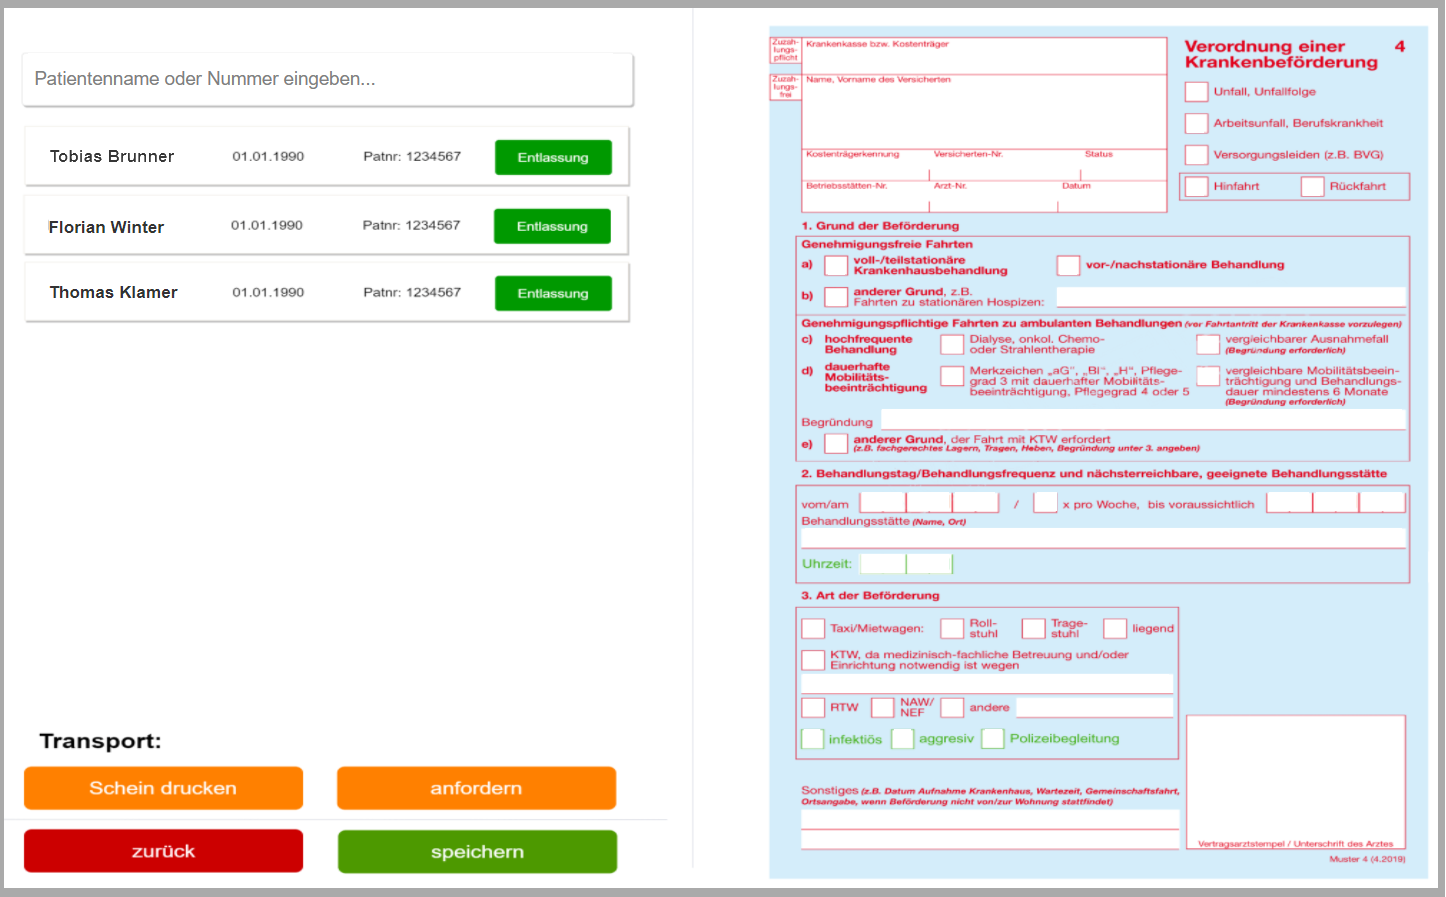
\includegraphics[width=\textwidth]{../Bilder/ap1Frame2.png}
	\captionof{figure}{Axure - Patientensuche und Transportschein}
	\label{img:ap1frame2}
\end{minipage}
\end{center}
Für die Erstellung eines neuen Transportes muss zunächst der zu entlassene Patient ausgewählt werden. Die Daten hierfür können der Patientendatenbank des Krankenhauses entnommen werden. Um den zu entlassenen Patienten schnell aufzufinden wird hier, wie bereits bei den Transporten, eine Suche nach Patientenname oder -nummer angeboten.\\

Beim Klick auf „Entlassung“ werden die Daten des Patienten aus der elektronischen Patientenakte in den Transportschein übernommen. Nun kann der Nutzer (Pflegepersonal) die restlichen Inhalte des Transportschein ausfüllen, die relevanten Inhalte an den Fuhrpark übermitteln und den Transportschein drucken. Der Transport wird gespeichert und anschließend auf der Startseite angezeigt.
\subsubsection{Modifizierter Transportschein}
\begin{center}
\begin{minipage}{0.8\textwidth}
	\centering
	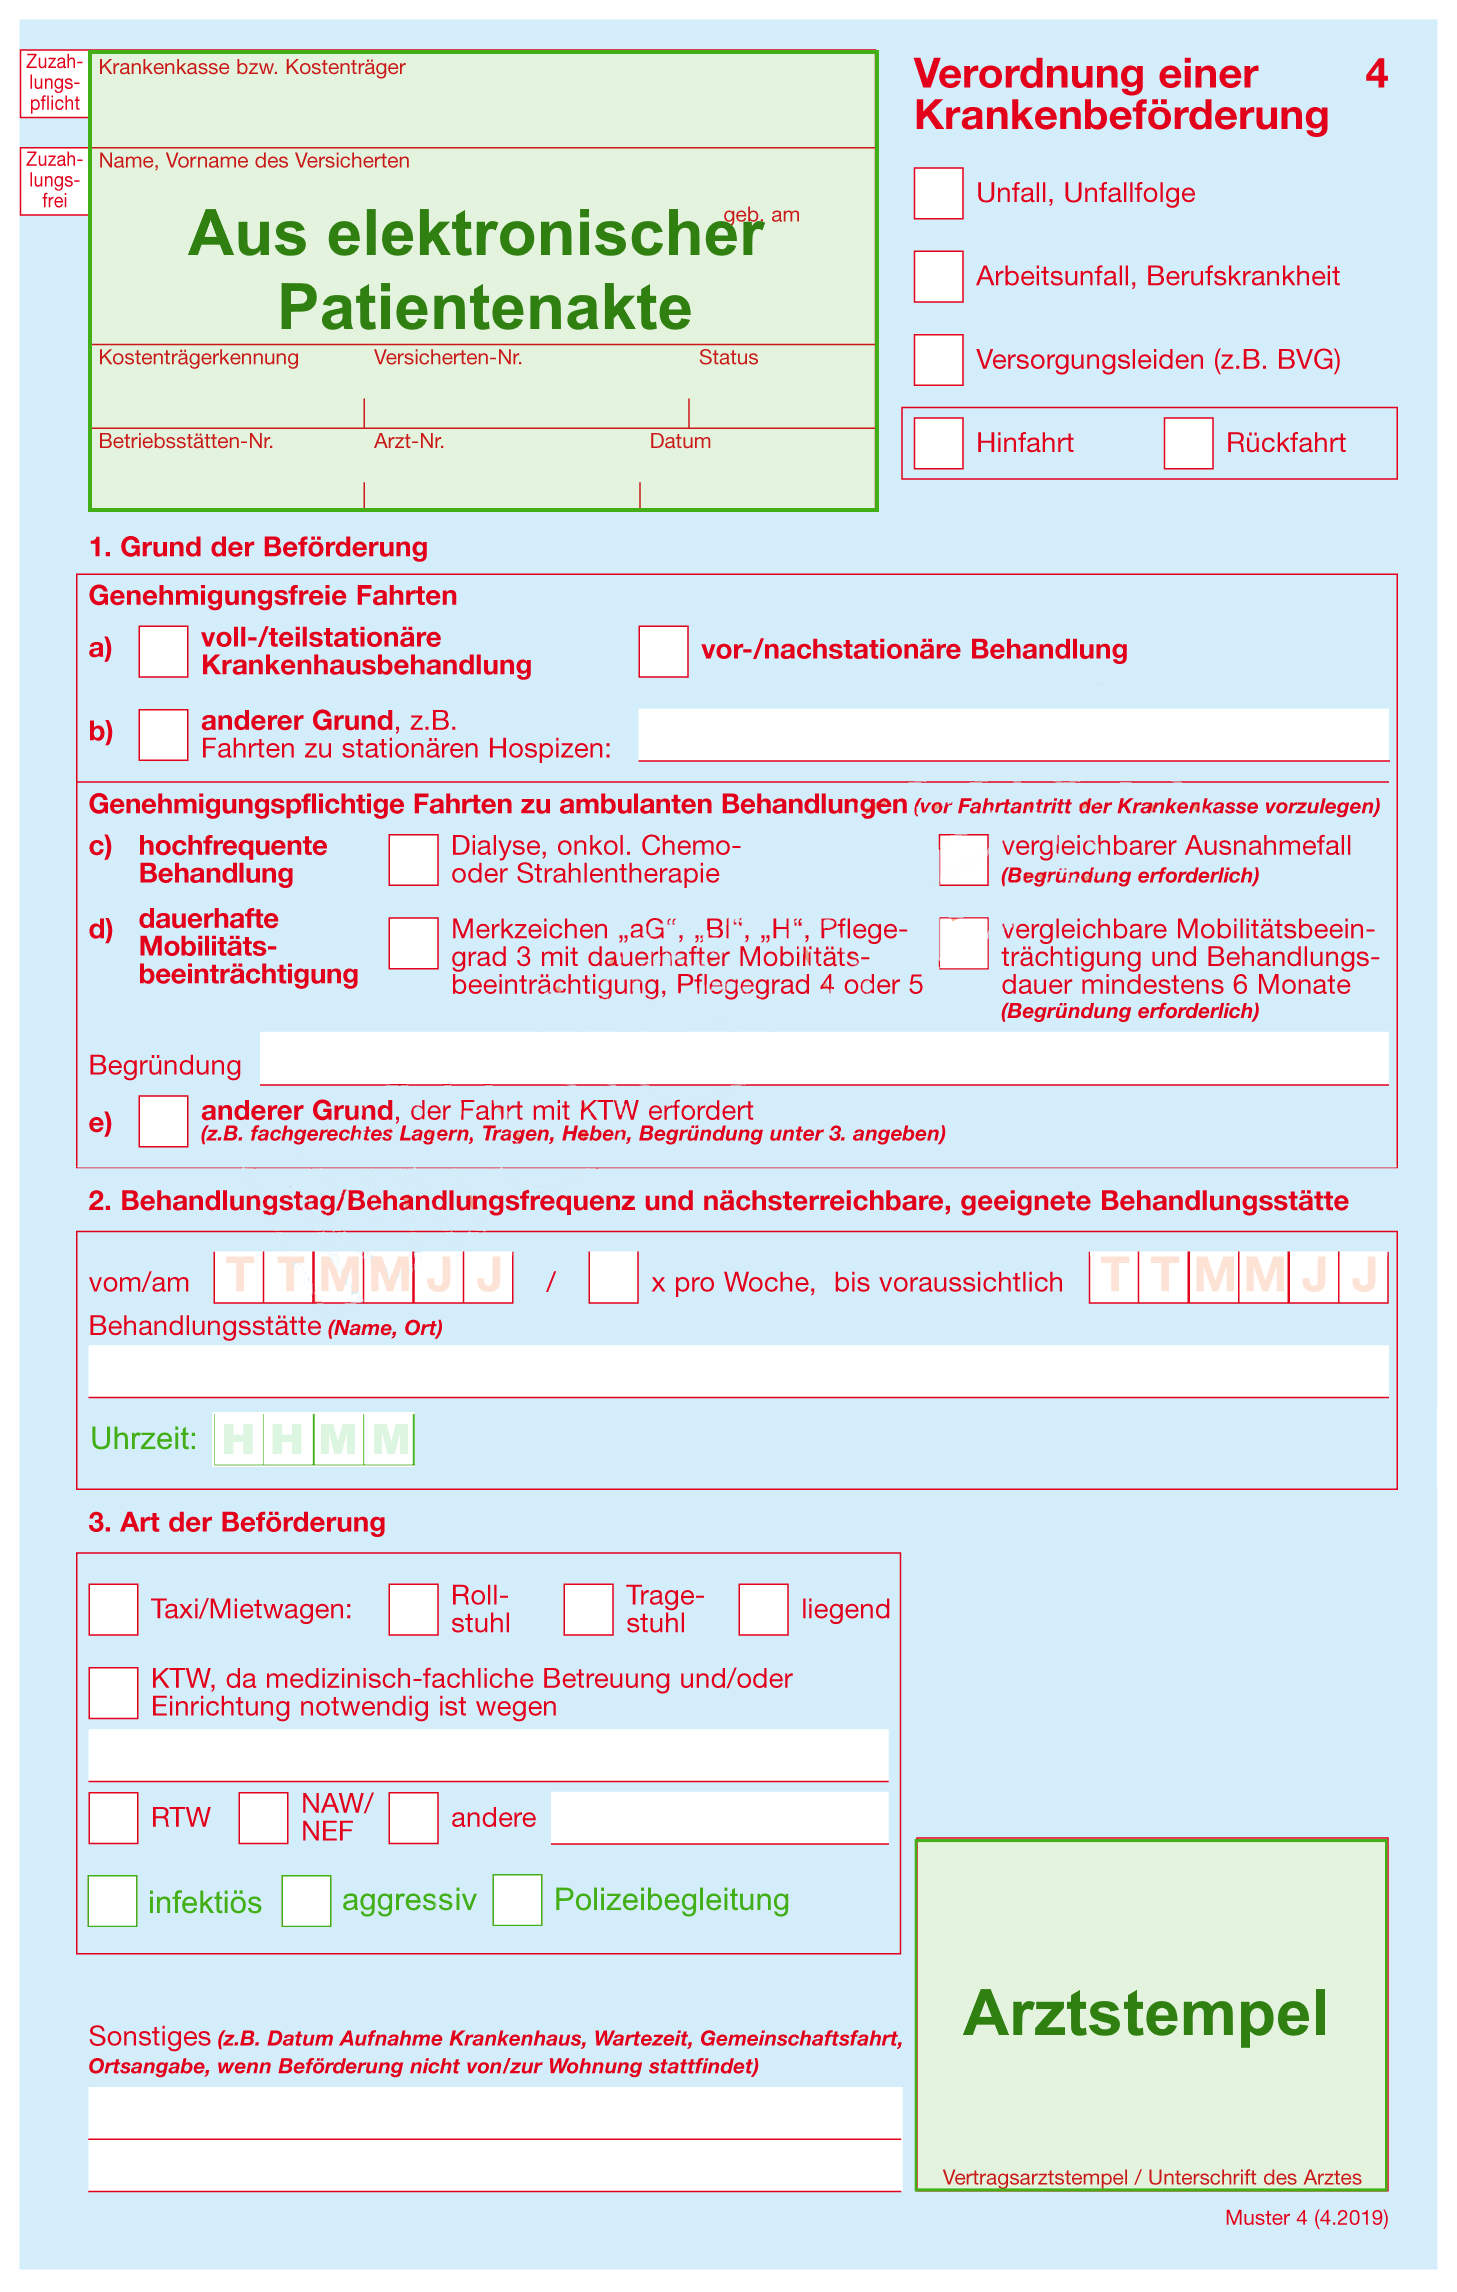
\includegraphics[width=\textwidth]{../Bilder/Krankentransportmodifiziert.png}
	\captionof{figure}{Axure - Modifizierter Transportschein}
	\label{img:Krankentransportmodifiziert}
\end{minipage}
\end{center}
Alle für einen Patiententransport relevanten Daten werden können in der Vorlage „Verordnung einer Krankenbeförderung“ der Kassenärztlichen Bundesvereinigung eingetragen werden. Wir haben uns dafür entschieden diese Vorlage in unseren Prototypen zu übernehmen, da unsere Zielnutzer (Pflegepersonal) an diesen gewöhnt sind und für den Transporteuer immer ausgedruckt werden muss.\\

Wir mussten allerdings feststellen, dass der Transportschein u.a. keine Eingabemöglichkeit für die genaue Uhrzeit des Termins bietet. Für die automatisierte Planung von Transporten sind außerdem noch andere relevante Informationen über den Patienten von Bedeutung (infektiös, aggressiv, …). Diese müssten im Transportschein als Freitext eingetragen werden und wären somit schwer weiterzuverarbeiten.\\

Wir haben uns deshalb dafür entschieden den Transportschein um ein paar Eingabemöglichkeiten zu erweitern. Das Originaldesign haben wir beibehalten, unsere zusätzlichen Eingabefelder unterscheiden sind lediglich farblich vom Original. Beim Ausdrucken des Transportscheins werden die Inhalte unserer hinzugefügten Eingabefelder in die bereits bestehenden optionalen Felder übernommen (andere, Sonstiges).
\subsection{Prototyp Vorstellung (Evaluieren der Gestaltungslösung anhand der Nutzungsanforderung) }
\subsubsection{St. Josef}
\colorbox{yellow}{tbi}\\
\subsubsection{Bezirksklinikum}
\colorbox{yellow}{tbi}\\
\subsection{Feedback aus den Krankenhäusern}
\subsubsection{Usetest Bezirksklinikum}
Am 17.12.2019 trafen sich Sebastian Brunner, Felix Richter und Tobias Winter aus unserer Gruppe erneut mit zwei anderen Teams im Bezirksklinikum Regensburg, um ihre jeweiligen Prototypen vorzustellen.\\

Leider war Frau Knopf zu diesem Termin im Krankenstand, daher wurden wir an Frau Traurig verwiesen. Frau Traurig ist im Bezirksklinikum Pflegedienstleiterin und hatte bedauerlicherweise mit der operationellen Seite auf Station keinerlei weitergehende Erfahrung.\\
 
Vor dem Usertest wurden folgende Szenarien ausgearbeitet, die den Anwendern sowohl die häufigsten Usecases, als auch neue und gegenüber dem jetzigem System erweiterte Funktionalität demonstrieren sollten:

\paragraph{Fall 0:}\leavevmode\\
Dieser Anwendungsfall sollte dem Benutzer Zeit geben, einen ersten Überblick über die Oberfläche zu erhalten und ihm gleichzeitig die Angst nehmen, mit dem Prototypen zu interagieren.\\
 
Aufgabe: “Die Transporte sind in verschiedene Stati (“alle”, “noch nicht angenommen”, “angenommen” und “storniert”) unterteilt. Bitte filtern Sie einmal nach jeder Kategorie.”\\
 
Resultat: Frau Traurig war etwas irritiert, da anfänglich keinerlei Transporte eingetragen waren und diese erst durch einen Klick auf “alle” erschienen sind. Nachdem alle Transporte eingeblendet wurden, musste sich erstmal ein Überblick über die angezeigten Informationen verschafft werden.\\
 
Mögliche Verbesserungen: Der anfangs nötige Klick auf “alle” war ein Designfehler unseres Prototypen. Eine überarbeitete Version zeigt standardmäßig die Ansicht aller Transporte an.

\paragraph{Fall 1:}\leavevmode\\
Aufgabe: “Bitte suchen Sie nach Florian Winter und bearbeiten Sie diesen Transport”\\
 
Resultat: Aufgabe nach anfänglichem Problem die Suchleiste zu lokalisieren problemlos gemeistert.

\paragraph{Fall 2:}\leavevmode\\
Aufgabe: ”Der Patient Tobias Brunner soll am 20.12.19 zur REHA gebracht werden. Die Entlassung ist schon sicher. Der Transport kann bereits angefordert werden. Der Patient soll im Taxi mit Rollstuhl transportiert werden.”\\
 
Resultat: Nach Auswahl von “neuer Transport” → “Case1” erste Unklarheit wegen der Betitelung der der Buttons links mit “Entlassung”. Button “ePA” zum Autoimport der Patientendaten aus der elektronischen Krankenakte nicht gefunden. Nach dem Import Unklarheit was Button “anfordern” bewirkt.\\

Mögliche Verbesserungen: Buttons mit Subjekt und Prädikat versehen. Statt “Entlassung” z.B. “Patientendaten importieren”. Import automatisch bei Klick auf “Patientendaten importieren” starten um zusätzlichen Doppelklick auf “ePA” zu vermeiden. Buttonbeschriftung “Patiententransport  anfordern” statt nur “anfordern”.\\
 
Aufgabe Teil 2: “Der Patient wurde abgeholt und der Auftrag kann nun mit einem Klick auf "erledigt" abgeschlossen werden.”
[Wegen der Beschränkungen von Axure war zur Simulation der verstrichenen Zeit ein Klick auf “Warte auf Bestätigung” notwendig, was der Probandin gesagt wurde]\\
 
Resultat: Frau Traurig konnte nicht nachvollziehen, warum ein Klick auf Warte auf Bestätigung” notwendig war. Auch was ein Klick auf “erledigt” auslöst war ihr nicht bewusst.\\
 
Mögliche Verbesserungen: Ansicht direkt auf Endzustand weiterleiten. Erledigte Aufträge automatisch ausblenden.

\paragraph{Fall 3:}\leavevmode\\
Aufgabe: “Florian Winter kommt zu einer Routine OP am 17.12.2019. Er soll voraussichtlich in zwei Tagen, am 19.12.2019 um 09:00 entlassen werden. Sie haben gerade Zeit und sollen vorab schon einmal die Daten eintragen und speichern. Der Patient soll liegend mit KTW transportiert werden.\\
 
Resultat: Frau Traurig hatte Probleme, das Formblatt für eine Krankenbeförderung auszufüllen. Sie arbeitet normalerweise nicht mit diesen Formblättern und hätte eine normale Eingabemaske bevorzugt. Unklarheit wegen der verschiedenen Stati eines Transportes (“erstellt”, “angefordert” und “erledigt”).\\
 
Es treten Probleme auf und der Patient soll nun sofort (am 17. um 18:00) entlassen werden. Der Patient soll hierbei mit dem RTW in ein anderes Krankenhaus verlegt werden. Liegendtransport mit RTW und infektiös soll angefordert werden. Der Transport wird vom RTW wegen Notfall abgesagt. Sie sollen den abgesagten Transport neu anfordern.”\\
 
Der letzte Teil konnte wegen Zeitmangels leider nicht mehr durchgespielt werden.\\
 
Im anschließenden Gespräch wurden von Frau Traurig noch einige weitere Punkte als besonders wichtig erwähnt. Eine Integration in das bestehende Krankenhaussystem “Nexus” sei äußerst wichtig, damit Nutzer sich nicht mit einem weiteren System auseinandersetzen müssen.\\

Des Weiteren sei das bestehende Nexus System sowie ein SAP System sehr unbeliebt, da beide dem Anwender gegenüber sehr hohe Latenzen aufweisen, was dem schnellen Ablauf von Aktionen in einer Krankenhausumgebung entgegensteht.\\
 
Diese beiden Punkte wären bei einer erneuten Iteration auf jeden Fall priorisiert zu berücksichtigen.

\paragraph{Fazit nach dem Usertest:}\leavevmode\\
Axure ist mit Sicherheit ein gutes Tool für Benutzer, die wenig bis keine Programmiererfahrung haben. Unserer Meinung nach ist selbst nach gründlicher Einarbeitung in Axure kein nennenswerter Geschwindigkeitsvorteil bei der Erstellung von Prototypen gegenüber z.B. einer Website festzustellen, vielmehr haben sich die Limitationen des Prototypen aufgrund von Axure als in der Praxis störend erwiesen.\\

Aufgrund der nur teilweise implementierten oder sinngemäß abgebildete Funktionen konnte sich der Benutzer nicht wirklich vorstellen, wie ein vollständig funktionierendes System arbeiten würde. Dies ist selbstverständlich auch dem generell nicht besonders ausgeprägtem Technikverständnis und der fehlenden Affinität des Personals zu neuen Prozessen geschuldet.
\section{Finaler Axure Prototyp}
Die Startseite des Prototypen blieb, aufgrund des positiven Feedbacks, unverändert. Eine grundlegende Überarbeitung erfuhr die Ansicht für die Planung der Transporte.
\begin{figure}[h]
\centering
\subfloat[][]{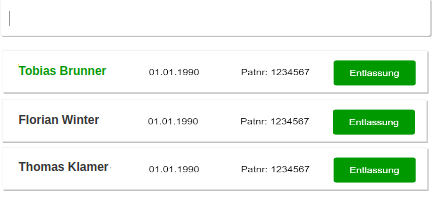
\includegraphics[width=0.32\textwidth]{../Bilder/patsearch1.png}}
\subfloat[][]{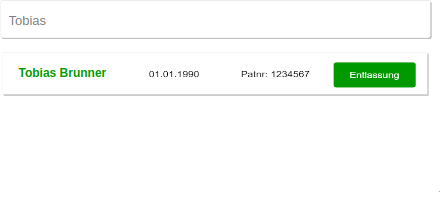
\includegraphics[width=0.32\textwidth]{../Bilder/patsearch2.png}}
\subfloat[][]{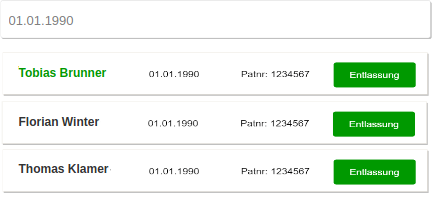
\includegraphics[width=0.32\textwidth]{../Bilder/patsearch3.png}}
\caption{Finaler Prototyp - Patientensuche}
\label{img:patsearch}
\end{figure}
Auf der linken Seite wurde die Suchfunktion für Patienten angepasst. Aufgrund des Nutzerverhaltens ist es zusätzlich zur Suche nach dem Patientennamen auch möglich Patienten nach ihrem Geburtsdatum zu druchsuchen.
\begin{center}
\begin{minipage}{0.8\textwidth}
	\centering
	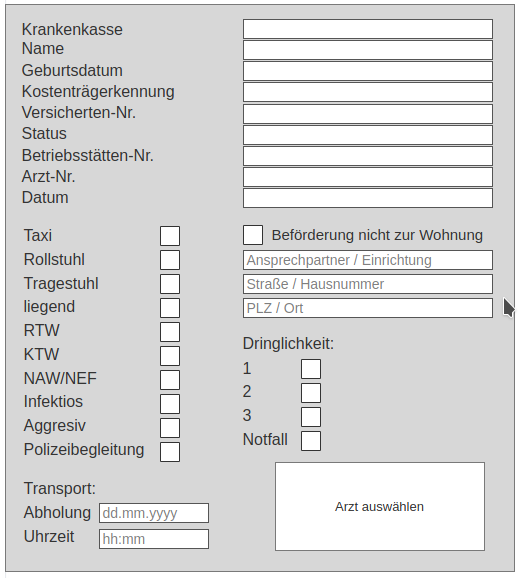
\includegraphics[width=\textwidth]{../Bilder/form.png}
	\captionof{figure}{Finaler Prototyp - Formular}
	\label{img:form}
\end{minipage}
\end{center}
Auf der rechten Seite wurde das Transportformular grundlegend überarbeitet. Aufgrund der besseren Lesbarkeit und Übersicht wurde auf den Schein ``Verordnung einer Krankenbeförderung'' verzichtet. Da viele Formularfelder des Scheins nicht benötigt wurden, griff man zu einem vereinfachten Formular mit essentiellen Feldern. Hinzugefügt wurden außerdem die Möglichkeit den Transport an einen anderen Bestimmungsort als die Patientenwohnung zu planen und die Einstufung des Transportes nach Dringlichkeit bis hin zum Notfall.\\
\begin{center}
\begin{minipage}{\textwidth}
\centering
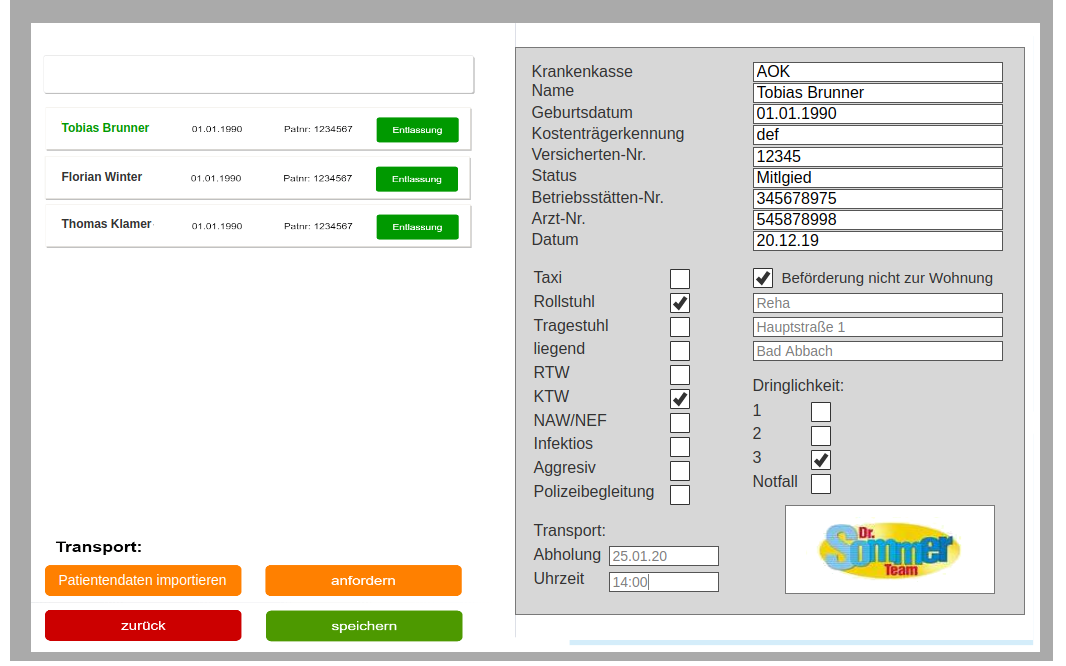
\includegraphics[width=\textwidth]{../Bilder/pat1.png}
\captionof{figure}{Finaler Prototyp - Patientendaten}
\label{img:pat}
\end{minipage}
\end{center}
Abbildung~\ref{img:pat} veranschaulicht den gesamten Prozess. Links wurde der Patient ``Tobias Brunner'' ausgewählt. Die Patientendaten wurden aus der elektronischen Patientenakte importiert (Button: ``Patientendaten importieren'') und der Rest des Formulars wurde händisch ausgefüllt. Zum Schluss wird noch der Arztstempel importiert. Die ausgefüllten Daten werden gespeichert. Wechselt man nun auf einen anderen Patienten und im Anschluss wieder zurück auf ``Tobias Brunner'' bleiben alle Daten erhalten. Lediglich der Arztstempel muss no aufgedruckt werden, da Änderungen zwischenzeitlich erfolgt sein können.
\section{Fazit}

\end{document}

